\chapter{Waves}

Wave is a way of transferring and storing \emph{energy} without the transport of matter. Most familiar examples are surface waves on water, sound waves, light waves. In the next two chapters, we are going to look at the basics of wave motion and some of the most important wave phenomena.

%Wave motion is the propagation of disturbance -- deviations from a state of equilibrium -- from one place to another. 
%
%Waves consist of continuous oscillations around some fixed locations.
%
%There are mainly two types of waves, \keypoint{mechanical waves} and \keypoint{electromagnetic waves}. Mechanical waves propagate as oscillations of matter, thus it must travel through a \emph{medium}. Electromagnetic waves can travel in free space.
%
%A wave can either be \keypoint{transverse} or \keypoint{longitudinal} depending on the direction of its oscillation. The direction of propagation of a transverse wave is perpendicular to the direction of its oscillation, and the wave motion of a longitudinal wave is parallel to its oscillation.

\subsection{wave terminologies}

wave motion is the propagation of disturbance from one place to another

\begin{figure*}[ht]
	\centering
	\begin{tikzpicture}[xscale=1.2, yscale=0.95]
	\draw [->] (0,-2) -- (0,2.4) node[midway,left]{$O$} node[above]{displacement};
	\draw [->] (0,0) -- (3.1*pi,0) node[below]{position};
	\draw[very thick,->] (1.8*pi,2) -- (2.6*pi,2);
	\node[above,twoline] at (2.2*pi, 2.1) {direction of\\wave motion};
	\foreach \t/\labelcolor in {1/{blue}, 2/{Green}, 3/{purple}, 4/{gray}} {
		\draw[\labelcolor] ({0.4*pi+(\t-1)*0.6)}, 1.7) --++ (0.2,0.5) node[above]{$t_\t$};
		\draw [thick, \labelcolor, domain=0:3*pi, samples=30, smooth] plot (\x,{1.6*sin((\x+0.6-0.6*\t)*1.25 r)});
	}
	\end{tikzpicture}
	
	\caption{wave pattern at different times ($t_1<t_2<t_3<t_4$) as wave travels in space}
\end{figure*}


to describe the wave motion and particle vibrations, we can define the following quantities:


\cmt as a wave moves out, each point oscillates back and forth about their rest positions

distance from a particle's equilibrium position is called \keypoint{displacement} of the particle \index{displacement}

\cmt greatest displacement for a particle is called the \keypoint{amplitude} ($A$) \index{amplitude}

\cmt wave pattern repeats itself over a certain distance

distance between two adjacent points undergoing exactly same motion is the \keypoint{wavelength} ($\lambda$) \index{wavelength}

one can think of wavelength as crest-to-crest distance, trough-to-trough distance, etc.\footnote{For now, we take for granted that a wave is transverse. There are also longitudinal waves for which terms like crest and trough do not apply. We will get into that in \S\ref{ch-Lwaves}.}

\cmt each point also repeats its vibrational motion over a certain time interval

time for a particle to complete a full oscillation cycle is the  \keypoint{period} ($T$) \index{period}

\cmt number of oscillations for a particle per unit time is the \keypoint{frequency} ($f$) \index{frequency}

frequency can also be defined as the number of crests passing a given point per unit time

frequency of a wave is related to its period by \begin{empheq}[box=\tcbhighmath]{equation*}{f=\frac{1}{T}}\end{empheq}

unit of frequency: $[f] = \text{Hz}$ (hertz), where $1 \text{ Hz} = 1 \text{ s}^{-1}$

\begin{figure*}[ht]
	\centering
	\begin{minipage}{0.48\textwidth}
		\centering
		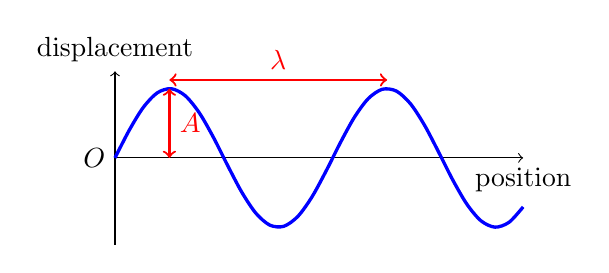
\begin{tikzpicture}[scale=0.55]
		\draw [->] (0,-2) -- (0,2) node[midway,left]{$O$} node[above]{displacement};
		\draw [->] (0,0) -- (3*pi,0) node[below]{position};
		\draw [very thick,blue,domain=0:3*pi,samples=30,smooth,variable=\x] plot (\x,{1.6*sin(\x*1.25 r)});
		\draw[<->, thick, red] (.4*pi,1.6) -- (.4*pi,0) node[midway,right]{$A$};
		\draw[<->, thick, red] (.4*pi,1.8) -- (2*pi,1.8) node[midway,above]{$\lambda$};
		\end{tikzpicture}
		
		wave pattern of all particles at one instant
	\end{minipage}\hfil
	\begin{minipage}{0.48\textwidth}
		\centering
		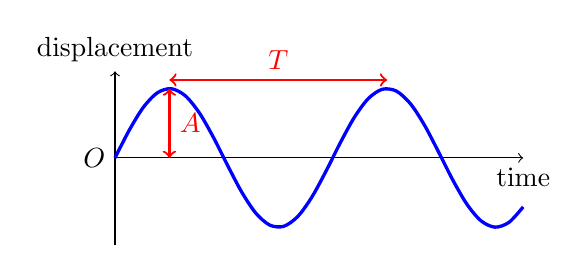
\begin{tikzpicture}[scale=0.55]
		\draw [->] (0,-2) -- (0,2) node[midway,left]{$O$} node[above]{displacement};
		\draw [->] (0,0) -- (3*pi,0) node[below]{time};
		\draw [very thick,blue,domain=0:3*pi,samples=30,smooth,variable=\x] plot (\x,{1.6*sin(\x*1.25 r)});
		\draw[<->, thick, red] (.4*pi,1.6) -- (.4*pi,0) node[midway,right]{$A$};
		\draw[<->, thick, red] (.4*pi,1.8) -- (2*pi,1.8) node[midway,above]{$T$};
		\end{tikzpicture}
		
		vibration of one specific particle at all times
	\end{minipage}
\end{figure*}

\cmt wave energy is transferred along the direction of wave motion at a certain speed $v$

in one period, wave moves forward by a distance of one wavelength

so \keypoint{wave speed} \begin{empheq}[box=\tcbhighmath]{equation*}{v=\frac{\lambda}{T}}\end{empheq}, or in terms of frequency, \begin{empheq}[box=\tcbhighmath]{equation*}{v=\lambda f}\end{empheq}

\example{When a wave travels on a water surface, the maximum depth of water is 21 cm and the minimum depth is 18 cm. What is the amplitude of the wave?}

\begin{soln} amplitude is half the end-to-end distance: $ A = \frac{1}{2}(21-18) = 1.5 \text{ cm} $ \end{soln}


\example{A wave travelling at $4.0 \mps$ has a wavelength of 50 cm, what is its period?}

\begin{soln} \begin{equation*}
	v = \frac{\lambda}{T} \RA T = \frac{\lambda}{v} = \frac{0.50}{4.0} = 0.125 \text{ s} 
\end{equation*}
\end{soln}

\subsection{transverse \& longitudinal waves}

a wave can either be \emph{transverse} or \emph{longitudinal}, depending on the direction of its oscillation

\subsection{transverse waves}

\begin{ilight}
	\centering a \keypoint{transverse} wave has vibrations at right angle to its direction of energy transfer \index{transverse wave}
\end{ilight}

\cmt examples of transverse waves: wave on a string, surface wave on water, light wave, etc.

\cmt for a transverse wave, greatest displacement in positive direction is called a \emph{crest}, or a \emph{peak}

greatest displacement in negative direction is called a \emph{trough}


\subsection{longitudinal waves} \label{ch-Lwaves}

\begin{ilight}
	\centering a \keypoint{longitudinal} wave has vibrations in parallel direction to energy transfer \index{longitudinal wave}
\end{ilight}

\cmt examples of longitudinal waves: sound waves, wave along a stretched slinky, etc.

\cmt for a longitudinal wave, if medium gets squeezed, we say this region is a \emph{compression}

if a medium expands, we say this region is a \emph{rarefaction}

\cmt wavelength of a longitudinal wave can be defined as compression-to-compression distance

\begin{figure*}[ht]
	\centering
	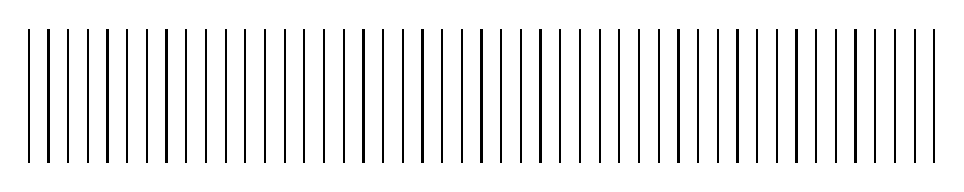
\begin{tikzpicture}[xscale=1, yscale=1.7]
	\foreach \x in {-0.75,-0.5,...,10.75}
	\draw[thick] ({\x} , -1) --++ (0,1);
	\end{tikzpicture}
	
	all particles at their equilibrium position before a pressure wave is set up
\end{figure*}

\begin{figure*}[ht]
	\centering
	\begin{tikzpicture}[xscale=1, yscale=1.7]
	\foreach \x in {-0.75,-0.5,...,11} 
		\draw[thick] ({\x+0.5*cos(\x*0.5*pi r)} , -1) --++ (0,1);
	\foreach \x in {-0.5,-0.25,...,11.25} 
		\draw[thick] ({\x+0.5*cos((\x-1)*0.5*pi r)} , -2.5) --++ (0,1);
	\foreach \x in {-0.5,-0.25,...,11} 
		\draw[thick] ({\x+0.5*cos((\x-2)*0.5*pi r)} , -4) --++ (0,1);
		\foreach \x in {3,7} \node[Green] at (\x,-1.2) {\phantom{p}rarefaction\phantom{p}};
		\foreach \x in {1,5,9} \node[blue] at (\x,-1.2) {compression};
		\foreach \x in {0,4,8} \node[Green] at (\x,-2.7) {\phantom{p}rarefaction\phantom{p}};
		\foreach \x in {2,6,10} \node[blue] at (\x,-2.7) {compression};
		\foreach \x in {1,5,9} \node[Green] at (\x,-4.2) {\phantom{p}rarefaction\phantom{p}};
		\foreach \x in {3,7} \node[blue] at (\x,-4.2) {compression};
		\node at (-1.5,-0.5) {{\large $t_1$}};
		\node at (-1.5,-2) {{\large $t_2$}};
		\node at (-1.5,-3.5) {{\large $t_3$}};
		\draw[very thick,->] (2.8,0.3) -- (7.2,0.3);
		\node[above,twoline] at (5, 0.4) {direction of wave motion};
		\draw[thick,red,<->] (1,-0.5) -- (5,-0.5) node[above,pos=0.55]{$\lambda$};
	\end{tikzpicture}
	
	\caption{compression and rarefaction regions at different times ($t_1<t_2<t_3$)	as a longitudinal pressure wave travels in space}
\end{figure*}



\example{What is the distance between a compression and a rarefaction for a sound wave of frequency 550 Hz? (Speed of sound in air is about $330 \mps$.)}

\begin{soln}\begin{equation*}
	d = \frac{1}{2}\lambda = \frac{v}{2f} = \frac{330}{2\times 550} \RA d = 0.30 \text{ m} 
\end{equation*}
\end{soln}

\subsection{sound waves}

sound waves propagate via the compression and rarefaction of air (or other medium) \index{sound}

molecules near vibrating source is pushed away from rest positions and into their neighbours

neighbouring molecules then in turn push into their neighbours, and so on

the disturbance is transferred through the medium, forming a sound wave

\cmt sound waves are longitudinal
	
\begin{figure*}[ht]

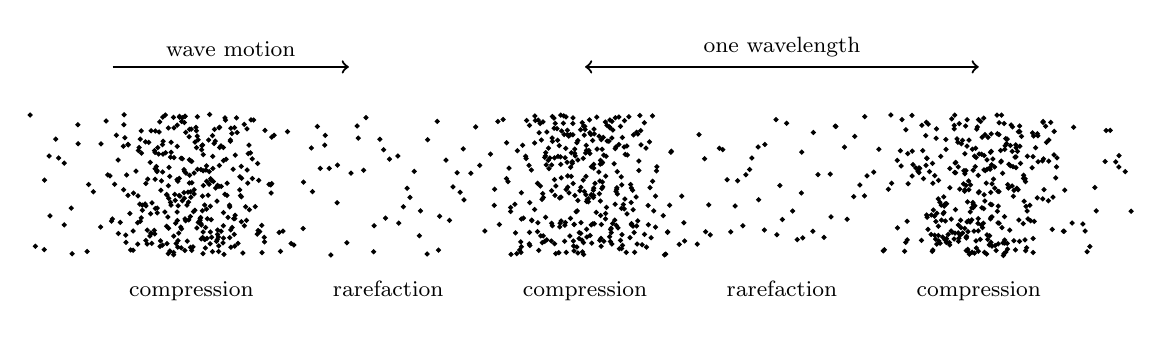
\begin{tikzpicture}[scale=1]
\pgfmathsetmacro{\noe}{6}

\foreach \t in {0,0.1,...,14}{
	\pgfmathsetmacro{\np}{pow({1+cos((\t-2)*pi/2.5 r)}, 4)*\noe/4}
	\foreach \idx in {0,1,...,\np} {
		\draw[fill] (\t+rnd*0.1-0.05,rnd*1.8) circle (0.025);	% wave 1
	}
}
\draw[<->,thick] (7,2.4) -- (12,2.4) node[midway,above]{{\footnotesize one wavelength}};
\draw[->,thick] (1,2.4) -- (4,2.4) node[midway,above]{{\footnotesize wave motion}};
\node[below] at (2,-.2) {{\footnotesize compression}};
\node[below] at (7,-.2) {{\footnotesize compression}};
\node[below] at (12,-.2) {{\footnotesize compression}};
\node[below] at (4.5,-.2) {{\footnotesize rarefaction}};
\node[below] at (9.5,-.2) {{\footnotesize rarefaction}};
\end{tikzpicture}
\end{figure*}

\cmt propagation of sound waves require medium (air, water, steel, etc.)
	
sound cannot travel in vacuum
	
\cmt speed of sound is material-dependent, but not frequency-dependent
	
	sound in general travels faster in denser medium
	
	\titem $v_\text{air} \approx 340 \mps$ (under standard atmospheric pressure and room temperature)
	
	\titem $v_\text{water} \approx 1500 \mps$
	
	\titem $v_\text{steel} \approx 5000 \mps$
	
\cmt \emph{pitch} of a note is related to frequency of sound wave

rapid vibrations of sound source at high frequencies produce a high pitch

\cmt \emph{loudness} of sound mainly depends on amplitude of vibration

a greater amplitude means the wave is more energetic so it sounds louder
	

\subsection*{measurement of sound waves}

two key apparatuses for sound measurement are the \keypoint{microphone} and the \keypoint{oscilloscope} \index{oscilloscope}

sound waves can be captured by a \emph{microphone}, which converts sound into electrical signals

electrical signals can then be sent into an \emph{oscilloscope} (see figure\footnote{The beautiful figure of the oscilloscope was created by \emph{Hugues Vermeiren}, who generously shared the source codes on TeXample: \url{http://www.texample.net/tikz/examples/textronics-oscilloscope/}}) for measurement

oscilloscope can be thought as an upgraded voltmeter showing how voltage varies with time

\begin{figure}[ht]
	\centering
	\includegraphics{oscilloscope.pdf}
	\caption{the display and controls of a typical cathode-ray oscilloscope}
\end{figure}

\cmt oscilloscope displays the variation of voltage ($y$-axis) with time ($x$-axis)

\cmt horizontal scale (time axis) is given by \emph{time-base} settings

vertical scale (voltage axis) is given by \emph{voltage gain}, or \emph{Y-sensitivity} settings

\cmt period $T$ of the sound wave can be found using time-base settings

then frequency of sound wave is calculated: $f=\frac{1}{T}$

\cmt voltage amplitude can be found using the voltage gain


\begin{marginfigure}
	\vspace*{-12pt}
	\centering
	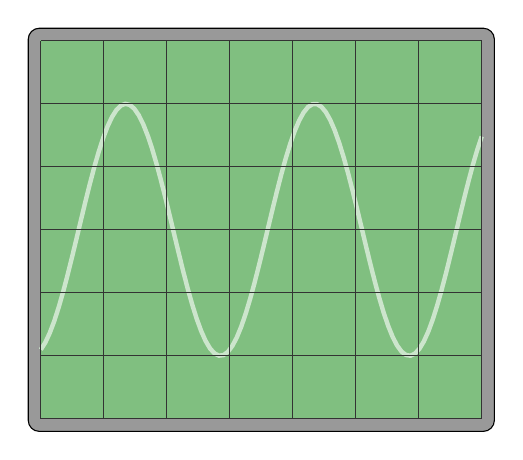
\begin{tikzpicture}[scale=0.8]
	\draw[fill=gray!80, rounded corners] (-0.2,-3.2) rectangle (7.2,3.2);
	\draw[Green!50, fill] (0,-3) rectangle (7,3);
	\draw[Green!20, ultra thick, domain=0:7, samples=100] plot (\x, {2*sin((\x-0.6)*120)});
	\draw[black!80, step=1] (0,-3) grid (7,3);
	\end{tikzpicture}
	\vspace*{-16pt}
\end{marginfigure}

\example{A sound wave is detected by a microphone and the trace is displayed on an oscilloscope as shown. If the time-base is set at 0.5 ms div$^{-1}$ and the voltage gain is set at 2 V div$^{-1}$. What is the frequency and the amplitude of the signal?}

\begin{soln} period: $T = 3 \times 0.5 \text{ ms} = 1.5 \times10^{-3} \text{ s}$

\eqyskip frequency: $f = \frac{1}{T} = \frac{1}{1.5 \times10^{-3} \text{ s}} \approx 667 \text{ Hz}$

\eqyskip amplitude: $A = 2 \times 2 \text{ V} = 4.0 \text{ V}$ \end{soln}




\subsection{electromagnetic waves}

a wave can be either \emph{mechanical} or \emph{electromagnetic}, depending on whether it requires a medium\index{electromagnetic wave}

\cmt waves that require a \emph{medium} to travel are called \keypoint{mechanical waves}

examples are sound waves, water waves, wave on a string, etc.

mechanical waves involve vibration of matter particles

\cmt no medium is needed for propagation of \keypoint{electromagnetic waves} i.e., they can travel in vacuum



\subsection{properties of electromagnetic waves}

\cmt electromagnetic waves can travel in free space

\cmt electromagnetic waves involve vibrations of electric and magnetic fields
	
an altering electric field can generate an altering magnetic field, which then further produces a new altering electric field, so on and so forth

electric and magnetic fields then permeate through space, transferring energy and information
	
\cmt electromagnetic waves are all transverse
	
vibration of electric fields and magnetic fields are both perpendicular to wave motion

\begin{figure*}[ht]
	\centering
	\begin{tikzpicture}[xscale=0.72]
	\draw[Green, thick, ->] (0,-2.1) -- (0,2.1) node[left, twoline] {electric\\field};
	\draw[blue, thick, dotted] (0 ,0) -- (0.7, 1.4);
	\draw[blue, thick, ->] (0, 0) -- (-0.7,-1.4) node[left, twolinecap] {magnetic\\field};
	\draw[thick, ->] (-0.3,0) -- (14,0) node[right, twoline]{direction\\ of energy\\transfer};
	\draw[Green, thick, domain=0:13.5, samples=150] plot (\x, {1.6*sin(2*\x r)});
	\draw[blue, thick] plot [smooth] coordinates {
		(0, 0)
		(0.0007, -0.1987)
		(0.0053, -0.3894)
		(0.0177, -0.5646)
		(0.0413, -0.7174)
		(0.0793, -0.8415)
		(0.134, -0.932)
		(0.2073, -0.9854)
		(0.3002, -0.9996)
		(0.4131, -0.9738)
		(0.5454, -0.9093)
		(0.6958, -0.8085)
		(0.8623, -0.6755)
		(1.0422, -0.5155)
		(1.2325, -0.335)
		(1.4294, -0.1411)
		(1.6292, 0.0584)
		(1.8278, 0.2555)
		(2.0213, 0.4425)
		(2.2059, 0.6119)
		(2.3784, 0.7568)
		(2.5358, 0.8716)
		(2.6758, 0.9516)
		(2.7968, 0.9937)
		(2.8981, 0.9962)
		(2.9795, 0.9589)
		(3.0417, 0.8835)
		(3.0864, 0.7728)
		(3.1156, 0.6313)
		(3.1323, 0.4646)
		(3.1397, 0.2794)
		(3.1415, 0.0831)
		(3.1417, -0.1165)
		(3.1442, -0.3115)
		(3.1529, -0.4941)
		(3.1715, -0.657)
		(3.2032, -0.7937)
		(3.2506, -0.8987)
		(3.316, -0.9679)
		(3.4007, -0.9985)
		(3.5053, -0.9894)
		(3.6296, -0.9407)
		(3.7727, -0.8546)
		(3.9328, -0.7344)
		(4.1075, -0.5849)
		(4.2939, -0.4121)
		(4.4886, -0.2229)
		(4.6876, -0.0248)
		(4.8872, 0.1743)
		(5.0832, 0.3665)
		(5.272, 0.544)
		(5.4499, 0.6999)
		(5.6139, 0.8278)
		(5.7614, 0.9228)
		(5.8905, 0.9809)
		(6, 1)
		(6.0896, 0.9792)
		(6.1597, 0.9193)
		(6.2114, 0.8228)
		(6.2468, 0.6935)
		(6.2683, 0.5366)
		(6.2791, 0.3582)
		(6.2828, 0.1656)
		(6.2832, -0.0336)
		(6.2842, -0.2315)
		(6.2899, -0.4202)
		(6.304, -0.5921)
		(6.3298, -0.7404)
		(6.3704, -0.8592)
		(6.4282, -0.9437)
		(6.5047, -0.9906)
		(6.601, -0.998)
		(6.7172, -0.9657)
		(6.8526, -0.8948)
		(7.0059, -0.7883)
		(7.1749, -0.6503)
		(7.3568, -0.4864)
		(7.5484, -0.3031)
		(7.7461, -0.1078)
		(7.946, 0.0919)
		(8.144, 0.2879)
		(8.3362, 0.4724)
		(8.5191, 0.6381)
		(8.6892, 0.7784)
		(8.8438, 0.8876)
		(8.9807, 0.9614)
		(9.0985, 0.9969)
		(9.1963, 0.9927)
		(9.2744, 0.9488)
		(9.3336, 0.8672)
		(9.3755, 0.751)
		(9.4024, 0.6048)
		(9.4173, 0.4346)
		(9.4235, 0.247)
		(9.4248, 0.0495)
		(9.4251, -0.1499)
		(9.4283, -0.3433)
		(9.4385, -0.5231)
		(9.459, -0.682)
		(9.4932, -0.8137)
		(9.5435, -0.9129)
		(9.6121, -0.9758)
		(9.7001, -0.9998)
		(9.808, -0.9839)
		(9.9356, -0.9288)
		(10.0817, -0.8367)
		(10.2444, -0.7112)
		(10.4213, -0.5573)
		(10.6094, -0.3813)
		(10.805, -0.19)
		(11.0044, 0.0089)
		(11.2037, 0.2073)
		(11.3988, 0.3976)
		(11.586, 0.5719)
		(11.7617, 0.7235)
		(11.9231, 0.8462)
		(12.0676, 0.9352)
		(12.1935, 0.9869)
		(12.2996, 0.9993)
		(12.3859, 0.9718)
		(12.4528, 0.9056)
		(12.5016, 0.8033)
		(12.5345, 0.6689)
		(12.5539, 0.5079)
		(12.5633, 0.3266)
		(12.5662, 0.1324)
		(12.5664, -0.0672)
		(12.568, -0.2641)
		(12.5748, -0.4504)
		(12.5906, -0.6188)
		(12.6187, -0.7626)
		(12.6621, -0.8759)
		(12.7229, -0.9543)
		(12.8027, -0.9946)
		(12.9023, -0.9954)
		(13.0218, -0.9564)
		};
	\end{tikzpicture}
	\caption{variation in electric and magnetic fields for an electromagnetic wave}
\end{figure*}

	
\cmt all electromagnetic waves travel at a constant speed $c=3.0\times10^8\mps$ in free space

i.e., speed of light in vacuum is constant\footnote{The speed of light in vacuum is actually a \emph{universal} physical constant. According to Einstein's special relativity, this is the upper limit for the speed at which matter and information can travel. This speed is also independent of the inertial reference frame one chooses, i.e., the speed of light in vacuum is the same for all observers, regardless of the motion of the source or the observer.}



\subsection{electromagnetic spectrum}

electromagnetic waves come in a wide range of wavelengths and frequencies 

distribution of electromagnetic radiation according to wavelength or frequency is the \keypoint{electromagnetic spectrum}\index{electromagnetic spectrum} (see diagram)



\begin{figure*}[!ht]
	\centering
	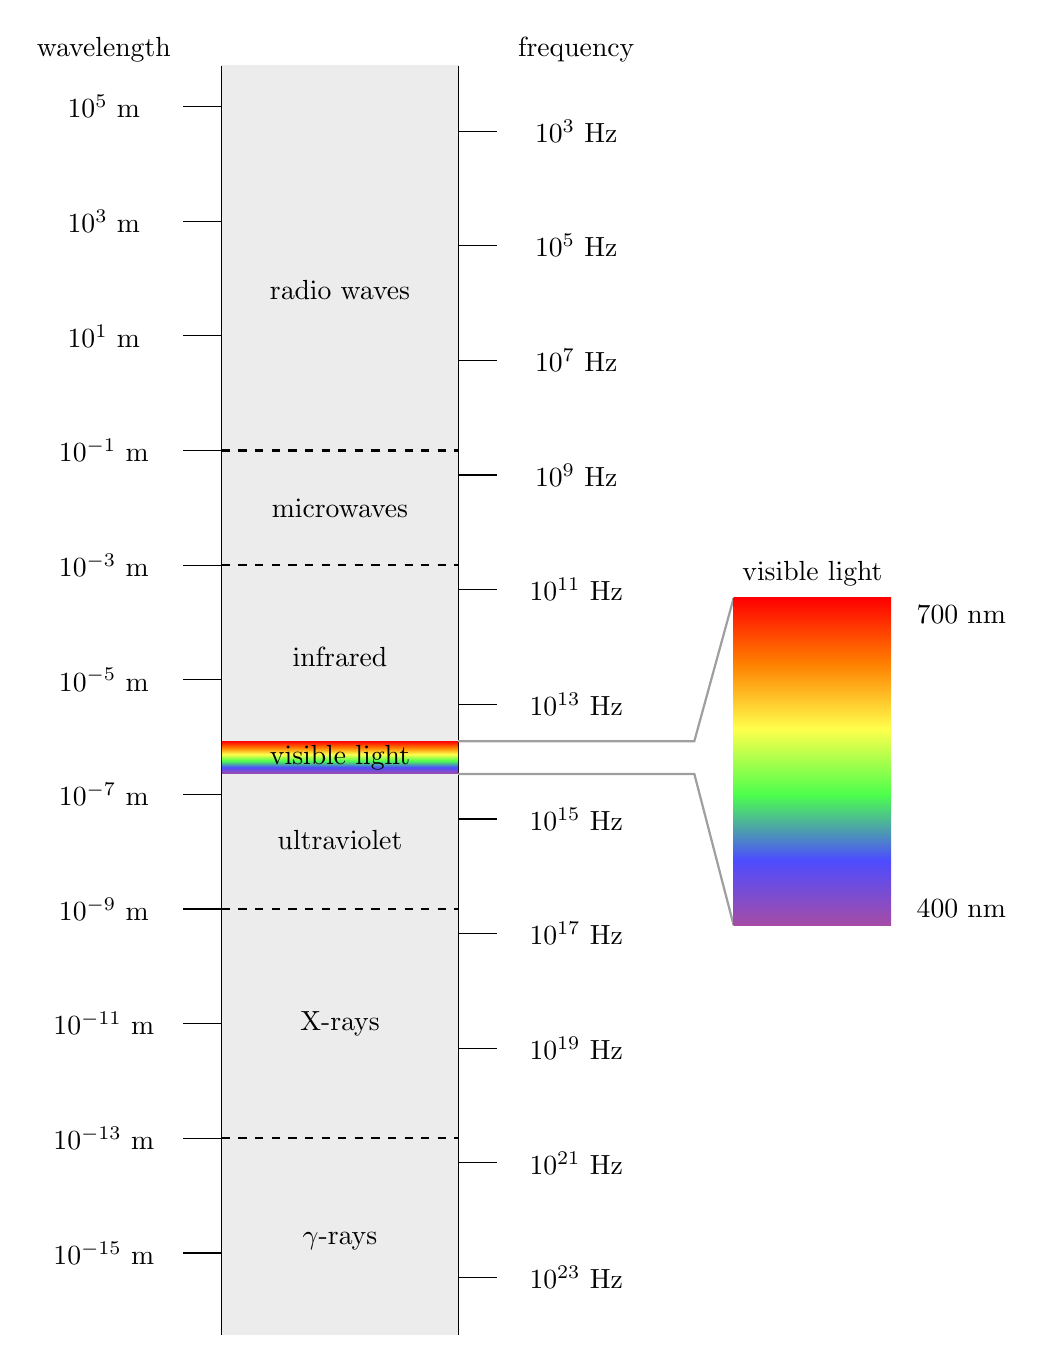
\begin{tikzpicture}[yscale=1.04]
	% define visible spectrum shading
	\pgfdeclareverticalshading{visible}{100bp}
	{color(0bp)=(violet!70); color(25bp)=(violet!70); color(35bp)=(blue!70);
		color(45bp)=(green!70); color(55bp)=(yellow!70); color(65bp)=(orange);
		color(75bp)=(red); color(100bp)=(red)}
	% grayish background for spectrum labels
	\draw[gray!15,fill] (-1.5,-8) rectangle (1.5,7.5);
	% axes
	\draw (-1.5,-8) -- (-1.5,7.5) (1.5,-8) -- (1.5,7.5);
	\node at (-3,7.7) {wavelength};
	\node at (3,7.7) {frequency};
	% spectrum labels
	\shade[shading=visible] (-1.5,-1.15) rectangle (1.5,-0.75);
	\foreach \x/\xlabel in {1.8/{radio waves}, -2/{microwaves}, -4.6/{infrared}, -6.35/{visible light}, -7.8/{ultraviolet}, -11/{X-rays}, -14.8/{$\gamma$-rays} } \node at (0,{\x*0.7+3.5}) {\xlabel};
	% values of wavelengths
	\foreach \x in {5,3,1,...,-15} {
		\draw (-1.5,{\x*0.7+3.5}) --++ (-0.5,0);
		\node at (-3,{\x*0.7+3.5}) {$10^{\x}$ m};
	}
	% values of frequencies
	\foreach \x in {3,5,...,23} {
		\draw (1.5,{-\x*0.7+8.8}) --++ (0.5,0);
		\node at (3,{-\x*0.7+8.8}) {$10^{\x}$ Hz};
	}
	% dashed lines as separators
	\foreach \x in {-1,-3,-9,-13} \draw[dashed,thick] (-1.5,{\x*0.7+3.5}) --++ (3,0);
	% extension for visible spectrum
	\draw[thick, gray!75] (1.5,-1.15) --++ (3,0) -- (5,-3);
	\draw[thick, gray!75] (1.5,-0.75) --++ (3,0) -- (5,1);
	\shade[shading=visible] (5,-3) rectangle (7,1);
	\node at (6, 1.3) {visible light};
	\node[right] at (7.2, 0.8) {700 nm};
	\node[right] at (7.2, -2.8) {400 nm};
	\end{tikzpicture}
	\caption{the electromagnetic spectrum}
\end{figure*}

\newpage

\cmt the table below shows electromagnetic spectrum in somewhat more precise details \footnote[][-2cm]{There are no precise accepted boundaries between different ranges in the electromagnetic spectrum. The boundaries are actually somewhat ambiguous. The ranges of different portions tend to overlap. For example, a large portion of the ranges of X-rays overlap with that of $\gamma$-rays, and microwaves are considered by many people as a subdivision of radio waves. Therefore, the values given here are merely supposed to give you some rough idea about the order of magnitudes for electromagnetic wavelengths and frequencies. So the point I want to make here is: do not take the borderlines too seriously.}
\vspace{3cm}
\begin{figure*}
\begin{center}
	\begin{tabular}{|C{4cm}|C{4cm}|C{4cm}|}
		\hline type of radiation & range of wavelength & range of frequency \\ 
		\hline radio waves  & 10$^{-1}$ $\sim$ 10$^{6}$ m & 10$^{2}$ $\sim$ 10$^{9}$ Hz \\ 
		\hline microwaves & 10$^{-3}$ $\sim$ 10$^{-1}$ m & 10$^{9}$ $\sim$ 10$^{11}$ Hz \\ 
		\hline infra-red & 7$\times$10$^{-7}$ $\sim$ 10$^{-3}$ m & 10$^{11}$ $\sim$ 10$^{14}$ Hz \\ 
		\hline visible light  & 4$\times$10$^{-7}$ $\sim$ 7$\times$10$^{-7}$ m & 10$^{14}$ $\sim$ 10$^{15}$ Hz \\ 
		\hline ultraviolet & 10$^{-9}$ $\sim$ 4$\times$10$^{-7}$ m & 10$^{15}$ $\sim$ 10$^{17}$ Hz \\ 
		\hline X-rays & 10$^{-13}$ $\sim$ 10$^{-9}$ m & 10$^{17}$ $\sim$ 10$^{19}$ Hz \\ 
		\hline $\gamma$-rays & 10$^{-16}$ $\sim$ 10$^{-11}$ m & 10$^{19}$ $\sim$ 10$^{24}$ Hz\\ 
		\hline
	\end{tabular} 
\end{center}
\end{figure*}

\cmt each type of electromagnetic waves has important applications in some area
\footnote{The entries listed here only include a teeny-weeny part of the uses of electromagnetic radiation, somewhat based on my personal taste. I also included a handful of explanations for the examples that I found interesting (otherwise I would not choose them), as you will see a huge load of footnotes in the next few pages. You are encouraged to do some researches as well, I can guarantee that you will not be disappointed.}

\begin{compactitem}
	\item[--] radio waves
	
	\xskip telecommunication (TV/radio broadcast, satellite communication) \footnote{Having the longest wavelengths of all radiation, radio waves have the best ability to diffract around obstacles in city buildings and mountains, therefore a large area can be covered.}

	\item[--] microwaves
	
	\xskip telecommunication (mobile phones, WiFi, Bluetooth, satellite communication)
	\footnote{Microwaves do not diffract sufficiently as radio waves, but they can transmit more information per unit time because they have higher frequencies. Microwaves are used in short-range telecommunication, including mobile phones, wireless networks, and bluetooth connections.}
		
		
	\xskip heating food (microwave ovens)
	\footnote{Frequency of microwaves are close to the natural frequencies of the rotational motion of water molecules. When food is exposed to microwaves, the water molecules in the food resonate and vibrate more violently, causing a rise in the food's temperature.}
	
	\item[--] infrared (IR)
	
	\xskip IR thermography (temperature monitors, thermographic cameras)
	\footnote{All objects emit electromagnetic radiation based on their temperatures. According to the law of black-body radiation, objects near room temperature emit thermal energy as infrared radiation, so variations in the temperature can be detected.}
	
	\xskip night-vision devices
	\footnote{Night-vision devices convert photons (just think of them as particles of light for now) into electrons, which are amplified by a chemical and electrical process and then converted back into visible light. Infrared sources can be used to augment the available light, increasing the visibility in the dark.}
	
	\xskip IR heating (IR heat lamps, IR saunas)
	
	
	\xskip IR data transmission (remote controls, optical-fibre communication)
	
	\item[--] visible light
	
	\xskip human vision
	\footnote{Human eyes are only sensitive to a small fraction of the electromagnetic spectrum. The wide variety of colours that we see is actually built up from the relative intensities of red, green and blue light collected by the three colour detectors in our eyes.}
	
	\item[--] ultraviolet (UV)
	
	\xskip UV sterilising (drinking water treatment, disinfection of medical facilities, etc.)
	\footnote{Short-wavelength UV light can damage the DNA's in living organisms. A microorganism exposed to germicidal UV light might not be able to reproduce, and becomes harmless. For the same reason, overexposure to UV radiation present in the sunlight can cause sunburn, or even skin cancer.}
		
	\xskip fluorescent dyes (black light fluorescent paint, UV watermarks)
	\footnote{UV radiation can cause many substances to glow through chemical reactions. UV watermarks that are visible under UV light are used to prevent counterfeiting of currency, or forgery of important documents such as passports and ID cards.}
	
	\item[--] X-rays
	
	\xskip medical imaging (X-ray imaging, CT scans)
	\footnote{X-rays are very energetic and thus very penetrating. They can pass through human body easily to form an image giving information about the structures of tissues and bones.}
	
	\xskip security check (luggage scanners)
	
	\xskip X-ray crystallography
	\footnote{X-rays can be diffracted by the lattice of atoms in a crystal. The diffraction pattern gives information about the structure of the lattice. X-ray crystallography is a very important experimental technique to study the microscopic structures of new materials.}
	
	\item[--] $\gamma$-rays
	
	\xskip radiation therapies (cancer treatment)
	\footnote{$\gamma$-rays have extremely high frequencies. They are even more energetic and penetrating. They can be used to damage the DNA of cancerous tissue, and hence kill the cancerous cells as a treatment.}
	
	\xskip medical imaging (PET scans)
	\footnote{Positron emission tomography (PET) uses a radioactive tracer to produce $\gamma$-rays within the tissues of interest. The energy and location of these $\gamma$-rays can be detected and sent to a computer to build up a 3D image of the body part.}
\end{compactitem}

\example{A beam of electromagnetic radiation is known to have a frequency of 25 THz in vacuum. What is its wavelength?}

\begin{soln}
    
\begin{equation*}
	\lambda = \frac{c}{f} = \frac{3.00\times10^8}{25\times10^12} \RA \lambda = 1.2 \times 10^{-5} \text{ m} \quad \text{(infra-red)} 
\end{equation*}
\end{soln}

	

\subsection{wave intensity}

energy can be transmitted along a wave

the degree to which energy is concentrated is called the intensity of the wave

here concentration has two meanings -- concentration in time and concentration in area $S$\footnote{To avoid confusion, I reserved letter `$A$' for wave amplitude and chose `$S$' to represent an area.}

\begin{ilight}
	\centering \keypoint{intensity} of a wave is defined as the power $P$ per unit area on a cross section $S$: \begin{empheq}[box=\tcbhighmath]{equation*}{I=\frac{P}{S}}\end{empheq}\index{wave intensity}
\end{ilight}

\cmt unit of wave intensity: $[I] = \text{ W m}^{-2}$

\cmt intensity is proportional to square of its amplitude: $\boxed{I \propto A^2}$.

\cmt intensity of a wave decreases as it spreads out in space

intensity at distance of $r$ from a point source is inversely proportional to $r^2$: $\boxed{I \propto \frac{1}{r^2}}$
\footnote{As a wave produced from a point source travels out by a distance $r$ away from the source, the energy it carries is spread uniformly over the surface area of the sphere of radius $r$, that is: $S=4\pi r^2$. So the intensity of a wave obeys an inverse square law: $I \propto \frac{1}{r^2}$.}

\example{If the amplitude of an incoming wave is increased by 50\%, what is the increase in the wave intensity?}

\begin{soln} $I \propto A^2 \RA \frac{I'}{I} = \left( \frac{A'}{A} \right)^2 = \left( 1 + 50\% \right)^2 =2.25 \RA $ so intensity is increased by 125\% \end{soln}

\example{Two observers $A$ and $B$ are at a distance $r_A$ and $r_B$ from a point source where $r_A=2r_B$. (a) Find the ratio of their intensities $\frac{I_A}{I_B}$. (b) Find the ratio of their amplitudes $\frac{A_A}{B_B}$.}

\begin{soln}

{
	\centering
	
	$ I \propto \frac{1}{r^2} \RA \frac{I_A}{I_B} = \left(\frac{r_B}{r_A}\right)^2 = \left(\frac{1}{2}\right)^2 \RA \frac{I_A}{I_B} = \frac{1}{4} $
	
	\vspace*{0.4em} $ I \propto A^2 \RA \frac{A_A}{A_B} = \sqrt{\frac{I_A}{I_B}} = \sqrt{\frac{1}{4}} \RA \frac{A_A}{A_B} = \frac{1}{2} $
	
}

\end{soln}




\subsection{polarisation}

\subsection{plane polarisation}

\begin{ilight}
	a wave is \keypoint{plane-polarised}, or simply \keypoint{polarised}, if the vibration is in one single direction at right angle to the direction of propagation of energy\index{polarisation}
\end{ilight}

\begin{figure}[ht]
	\centering
	\begin{minipage}{0.45\textwidth}
		\centering
		\begin{tikzpicture}[scale=0.64]
		\draw[very thick, blue, ->] (210:2) -- (30:8) node[twoline, above, black]{direction of\\energy transfer};
		\foreach \t in {0,45,90,135} {
			\draw[red, ultra thick, <->] (\t:1.5) --++ ({\t+180}:3);
			\draw[red, ultra thick, <->] (30:3.5) ++ (\t:1.5) --++ ({\t+180}:3);
		}
		\end{tikzpicture}
		
		an unpolarised wave
		
		(wave vibrations in multiple directions)
	\end{minipage}\hfil
	\begin{minipage}{0.45\textwidth}
		\centering
		\begin{tikzpicture}[scale=0.64]
		\draw[very thick, blue, ->] (210:2) -- (30:8) node[twoline, above, black]{direction of\\energy transfer};
		\foreach \t in {90} {
			\draw[red, ultra thick, <->] (\t:1.5) --++ ({\t+180}:3);
			\draw[red, ultra thick, <->] (30:3.5) ++ (\t:1.5) --++ ({\t+180}:3);
		}
		\end{tikzpicture}
		
		a plane-polarised wave
		
		(wave vibrations in one direction only)
	\end{minipage}
\end{figure}

\cmt polarisation\footnote[][-10cm]{Apart from plane polarisation where the vibrations are fixed in a single direction, there are also \emph{circular} or \emph{elliptical} polarisation, for which the direction of vibrations \emph{rotate} in a plane as the wave travels.} is a phenomenon associated with \emph{transverse} waves only

longitudinal waves (such as sound waves) cannot be polarised

this is because longitudinal vibrations are always parallel to direction of energy transfer

\cmt most important examples are polarisation of \emph{electromagnetic waves}

regarding vibration of electromagnetic waves, we usually focus on variations of electric field

\cmt sunlight, light emitted from incandescent bulbs are unpolarised

they are emitted randomly from their sources, so they contain all planes of polarisation


\cmt a few of the great many applications of polarisation are:

\begin{compactitem}
	\item[--] polarising sunglasses \& photography \sidenote[][-10cm]{When unpolarised light is reflected at the boundary of two media, the reflected beam would become partially polarised. Polarising sunglasses use this effect to reduce the sunlight reflected from shiny surfaces, such as a lake (for sightseeing tourists) or road surfaces (for drivers). For the same reason, photographers often place a polarising filter in front of the camera lens to darken skies and increase the contrast.}
	
	\item[--] polarised 3D films\footnote[][-6.5cm]{The eyeglasses worn by viewers contain a pair of polarising filters with mutually perpendicular axes. When two images are projected onto the same screen, each filter restricts the light reaching each eye by passing only one of the images that is polarised in the same direction. This creates an 3D illusion.}
	
	\item[--] liquid-crystal display (LCD) technology\footnote[][-4cm]{Liquid crystal arrays can be realigned by applying an electric field. This causes the axis of polarization to rotate, hence backlight may be allowed to pass or be blocked, forming dark patterns of the display.}
	
	\item[--] radio transmission and reception\footnote[][-2cm]{Since electric currents flow in certain directions only, so the radio waves and microwaves produced from aerials are intrinsically polarised. This means the reception of signals would be sensitive to a particular direction, but totally insensitive to the normal direction. This explains why altering the orientation of antennas could greatly enhance the quality of reception.}
\end{compactitem}

\subsection{polarisers \& Malus's law}

a plane-polarised light can be produced from unpolarised light using a \keypoint{polariser}

a polariser blocks vibrations in all planes except the plane of polarisation\footnote[][-2cm]{What we are discussing here is just one type of polariser, often called a \emph{linear absorptive polariser}, which is basically a synthetic transparent plastic sheet made of certain crystals. The thin sheet contains long-chain organic molecules aligned parallel to each other. When an unpolarised light passes through the polariser, there is a strong absorption of the electric field parallel to the alignment of molecules, so vibration of the electric field is allowed to pass in one direction only.}

direction along which vibration is allowed to pass is called the axis of the polariser

\begin{figure*}[ht]
	\centering
	\begin{tikzpicture}[scale=0.65]
	\draw[very thick, blue, ->] (0,0) -- (10,0);	
	\draw[fill=cyan!30] (0,0) ++ (0,2) ++ (160:2) --++ (-20:4) --++ (0,-4) --++ (160:4) --++ (0,4);
	\foreach \t in {-1.5,-1,...,1.5} \draw[very thin, gray!80, decorate, decoration={snake, amplitude=0.6}] (0,0) ++ (0,\t) ++ (160:1.6) --++ (-20:3.2);
	\draw[thick, Green, dashed] (0,1.8) -- (0,-1.8);
	\draw[Green] (0.1,1.2) -- (1.6,3) node[black, right, twoline]{axis of\\transmission};
	\draw[gray!80] (-1.4,1.6) -- (-3,3) node[black, left, twoline]{direction of alignment\\of molecules};
	\draw[very thick, blue] (-10,0) -- (0,0);
	\foreach \t in {-20,40,90,125} {
		\draw[red, ultra thick, <->] (-4,0) ++ (\t:1.5) --++ ({\t+180}:3);
		\draw[red, ultra thick, <->] (-8,0) ++ (\t:1.5) --++ ({\t+180}:3);
	}
	\foreach \t in {4,8} \draw[red, ultra thick, <->] (\t,-1.5) --++ (0,3);
	\node at (-6,-3.2) {unpolarised light};
	\node at (6,-3.2) {plane-polarised light};
	\node at (0,-3.2) {polariser};
	\end{tikzpicture}
	
	\caption{unpolarised light goes through a polariser and becomes plane-polarised}
\end{figure*}

\cmt polarised light can be sent through a second polarising filter (sometimes called an \emph{analyser})


\begin{figure*}[ht]
	\centering
	\begin{minipage}{0.45\textwidth}
		\centering
		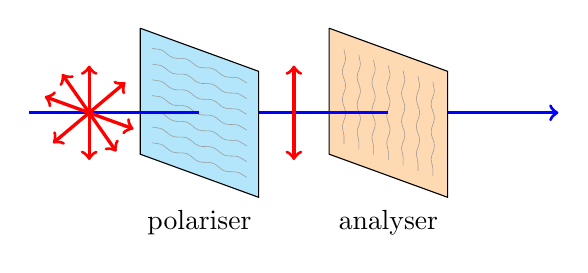
\begin{tikzpicture}[scale=0.4]
		\draw[very thick, blue, ->] (3,0) -- (8.4,0);	
		\draw[fill=orange!30] (3,0) ++ (0,2) ++ (160:2) --++ (-20:4) --++ (0,-4) --++ (160:4) --++ (0,4);
		\foreach \t in {-1.5,-1,...,1.5} \draw[very thin, gray!80, decorate, decoration={snake, amplitude=0.6}] (3,0) ++ (0,1.5) ++ (160:\t) --++ (0,-3);	
		\draw[very thick, blue] (-3,0) -- (3,0);	
		\draw[fill=cyan!30] (-3,0) ++ (0,2) ++ (160:2) --++ (-20:4) --++ (0,-4) --++ (160:4) --++ (0,4);
		\foreach \t in {-1.5,-1,...,1.5} \draw[very thin, gray!80, decorate, decoration={snake, amplitude=0.6}] (-3,0) ++ (0,\t) ++ (160:1.6) --++ (-20:3.2);	
		\draw[very thick, blue] (-8.4,0) -- (-3,0);
		\foreach \t in {-20,40,90,125} {
			\draw[red, very thick, <->] (-6.5,0) ++ (\t:1.5) --++ ({\t+180}:3);
		}
		\foreach \t in {0} \draw[red, very thick, <->] (\t,-1.5) --++ (0,3);
		\node at (-3,-3.5) {polariser};
		\node at (3,-3.5) {analyser};
		\end{tikzpicture}
		
		no transmission of light if polariser and 
		
		analyser are aligned at right angles
	\end{minipage}\hfil
	\begin{minipage}{0.45\textwidth}
		\centering
		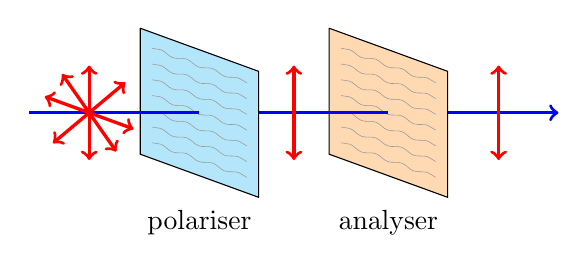
\begin{tikzpicture}[scale=0.4]
		\draw[very thick, blue, ->] (3,0) -- (8.4,0);	
		\draw[fill=orange!30] (3,0) ++ (0,2) ++ (160:2) --++ (-20:4) --++ (0,-4) --++ (160:4) --++ (0,4);
		\foreach \t in {-1.5,-1,...,1.5} \draw[very thin, gray!80, decorate, decoration={snake, amplitude=0.6}] (3,0) ++ (0,\t) ++ (160:1.6) --++ (-20:3.2);	
		\draw[very thick, blue] (-3,0) -- (3,0);	
		\draw[fill=cyan!30] (-3,0) ++ (0,2) ++ (160:2) --++ (-20:4) --++ (0,-4) --++ (160:4) --++ (0,4);
		\foreach \t in {-1.5,-1,...,1.5} \draw[very thin, gray!80, decorate, decoration={snake, amplitude=0.6}] (-3,0) ++ (0,\t) ++ (160:1.6) --++ (-20:3.2);	
		\draw[very thick, blue] (-8.4,0) -- (-3,0);
		\foreach \t in {-20,40,90,125} {
			\draw[red, very thick, <->] (-6.5,0) ++ (\t:1.5) --++ ({\t+180}:3);
		}
		\foreach \t in {0,6.5} \draw[red, very thick, <->] (\t,-1.5) --++ (0,3);
		\node at (-3,-3.5) {polariser};
		\node at (3,-3.5) {analyser};
		\end{tikzpicture}
		
		polarised light is unaffected if polariser
		
		and analyser are aligned in parallel
	\end{minipage}
\end{figure*}

\cmt if polarised light of initial intensity $I_0$ has an angle $\theta$ to the axis of analyser

\keypoint{Malus's law}\index{Malus's law} states that transmitted intensity is given by: ${I = I_0 \cos^2 \theta}$

this is because only electric field parallel to axis of analyser is transmitted

so transmitted amplitude\footnote{This is actually the amplitude of the electric field strength.} satisfies: $A = A_0 \cos\theta$, where $A_0$ is the initial amplitude

recall that intensity is proportional to square of amplitude, so $I = I_0 \cos^2 \theta $

\example{A beam of light polarised in the vertical direction has an amplitude $A$ and intensity $I$. It passes through a polarising filter whose axis of polarisation is at $45^\circ$ to the vertical. (a) What is the amplitude and the direction of polarisation of the emerging beam? (b) If the emerging beam then enters another filter whose axis of polarisation is at $75^\circ$ to the vertical, what is the amplitude and intensity of the emerging beam?}

\begin{soln} through first filter: 
$A_1 = A \cos\theta_1 = A \cos 45^\circ \RA A_1 = \frac{1}{\sqrt{2}} A $
light is polarised in a direction at $60^\circ$ to the vertical

through second filter:
$A_2 = A_1 \cos\theta_2 = \frac{1}{\sqrt{2}} A \times \cos (75^\circ - 45^\circ) \RA A_2 = \frac{\sqrt{6}}{4} A $

$I_2 = \left(\frac{\sqrt{6}}{4} \right)^2 I \RA I_2 = \frac{3}{8} I$

 or, $I_2 = I \cos^2\theta_1 \cos^2 \theta_2^2 = I \times \cos^2 45^\circ \times \cos^2 (75^\circ-45^\circ) \RA I_2 = \frac{3}{8} I$ 

\end{soln}





\subsection{diffraction}

a wave has the ability to bend around obstacles or pass through narrow gaps

\begin{ilight}
	when a wave passes through a aperture/slit/gap/hole or encounters an obstacle, it spreads out/around the corners, this is known as \keypoint{diffraction}\index{diffraction} of waves
\end{ilight}

\cmt diffraction is a general property of all waves

some examples of diffraction are

\begin{compactitem}
	\item[--] sound waves can diffract through an open door
	
	so you can hear people in the next room talking, even though you cannot see them
	
	\item[--] light ray can bend when it goes through/around a small hole/small particles
	
	sky appears red at sunset as red light is diffracted most by dust particles in atmosphere
\end{compactitem}

\cmt a wave is diffracted most when its wavelength is close to size of aperture/obstacle

a wave with longer wavelength usually diffracts more than a wave of shorter wavelength

\begin{figure*}[htp]
	\centering
	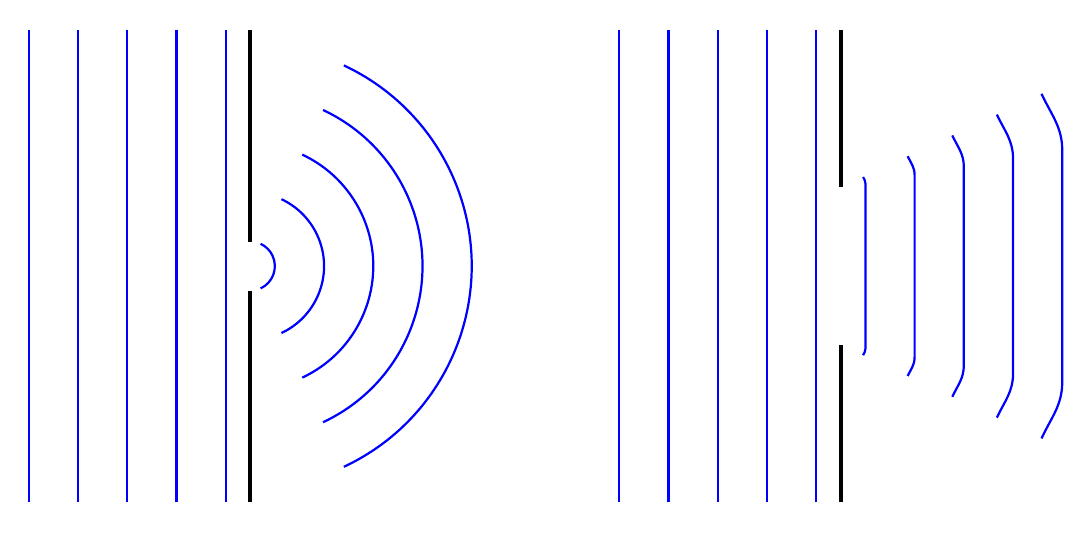
\begin{tikzpicture}[scale=1.25]
	\draw[ultra thick] (0,2.4) -- (0,0.25) (0,-0.25) -- (0,-2.4);
	\foreach \x in {0.25,0.75,1.25,1.75,2.25}{
		\draw[blue,thick] (-\x,-2.4) -- (-\x,2.4);
		\draw[blue,thick] (-65:\x) arc(-65:65:\x);
	}
	\draw[ultra thick] (6,2.4) -- (6,0.8) (6,-0.8) -- (6,-2.4);
	\foreach \x in {0.25,0.75,1.25,1.75,2.25}{
		\draw[blue,thick] (-\x+6,-2.4) -- (-\x+6,2.4);
		\draw[blue,thick] (6,-0.8) ++ (-25:\x) to[out=65,in=270] (6+\x,-0.8-\x/6) -- (6+\x,0.8+\x/6) to[out=90,in=-65] (6+0.9063*\x,0.8+0.4226*\x);
	}
	\end{tikzpicture}
	
	\caption{diffraction of a wave as it passes through an aperture of width that is (a) close to the wavelength, (b) greater than the wavelength}
\end{figure*}

\newpage


\subsection{Doppler effect}

\begin{ilight}
	relative motion between wave source and the observer causes a change in observed frequency, this is known as the \keypoint{Doppler effect}\index{Doppler effect}
\end{ilight}

\cmt any type of wave can exhibit Doppler effect

\cmt when wave source moves towards observer, a higher frequency is observed

when wave source moves away from observer, a lower frequency is observed

\cmt Doppler effect also occurs if source is at rest but observer is in motion

as long as there is \emph{radial} motion between source and observer, there is shift in frequency

\cmt Doppler effect finds its use in many areas, some examples are

\begin{compactitem}
	\item[--] \emph{Doppler radars}: used to measure velocity of moving target (speeding cars, tennis balls, etc.)
	
	\item[--] \emph{Doppler ultrasonography}: used to image blood flow in human bodies
	
	\item[--] \emph{astronomy}: used to study motion of stars and galaxies
\end{compactitem}

\newpage

\subsection*{explanation for Doppler effect}

suppose wave source is moving towards the observer at speed $v_s$

at time $t=0$, the source emits a wavefront which travels at speed $v$

\begin{figure*}[ht]
	\centering
	\begin{tikzpicture}[scale=0.95]
	\draw[thick] (0,0) circle (0.2);
	\draw[fill] (12,0.4) circle (0.2);
	\draw[ultra thick] (12,0.2) -- (12,-0.1) -- (11.8,-0.6) (12,-0.1) -- (12.2,-0.6) (11.75,-0.1) -- (12,0.15) -- (12.25,-0.1);
	\draw[blue,thick] (0.4, 0.62513) arc (10:-10:3.6);
	\node at (0,-1) {source};
	\node at (12,-1) {observer};
	\end{tikzpicture}
\end{figure*}

after one period, wavefront travels forward by a distance of $vT$

at same time, source moves forward by a distance of $v_s T$ and emits a new wavefront

\begin{figure*}[ht]
	\centering
	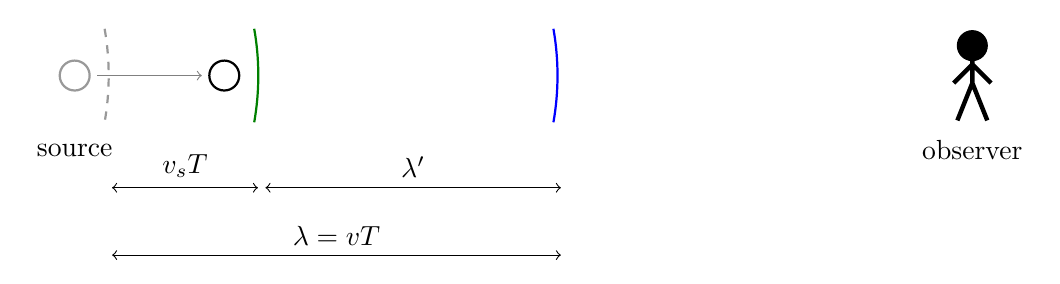
\begin{tikzpicture}[scale=0.95]
	\draw[thick,gray!80] (0,0) circle (0.2);
	\draw[thick] (2,0) circle (0.2);
	\draw[gray, ->] (0.3,0) -- (1.7,0);
	\draw[fill] (12,0.4) circle (0.2);
	\draw[ultra thick] (12,0.2) -- (12,-0.1) -- (11.8,-0.6) (12,-0.1) -- (12.2,-0.6) (11.75,-0.1) -- (12,0.15) -- (12.25,-0.1);
	\draw[Green,thick] (2.4, 0.62513) arc (10:-10:3.6);
	\draw[blue,thick] (6.4, 0.62513) arc (10:-10:3.6);
	\draw[gray!80,dashed,thick] (0.4, 0.62513) arc (10:-10:3.6);
	\node at (0,-1) {source};
	\node at (12,-1) {observer};
	\draw[<->] (2.55,-1.5) -- (6.5,-1.5) node[above, midway]{$\lambda'$};
	\draw[<->] (0.5,-1.5) -- (2.45,-1.5) node[above, midway]{$v_s T$};
	\draw[<->] (0.5,-2.4) -- (6.5,-2.4) node[above, midway]{$\lambda = vT$};
	\end{tikzpicture}
\end{figure*}

if source is at rest, observer simply perceives a wavelength $\lambda = vT$

now source is moving closer, a shorter wavelength $\lambda'$ is perceived

since frequency is inversely proportional to wavelength, so higher frequency $f'$ is observed

similar discussion follow for the case where source moves away from observer

\cmt change in observed frequency is due to change in wavelength caused by relative motion

if source moves towards/away from observer, apparent wavelength becomes shorter/longer

\subsection*{Doppler effect equation}

we are now ready to derive an equation for the shift of observed frequency

quantitatively, we can write: $\lambda' = \lambda \mp v_s T \quad$ ("$-$"/"$+$" if source is moving closer/away)

using $v = \lambda f$ and $f=\frac{1}{T}$, this becomes: $ \frac{v}{f'} = \frac{v}{f} \mp \frac{v_s}{f} $

rearranging, one finds observed frequency is given by: $\boxed{f' = f\frac{v}{v \mp v_s}}$

\example{A police car moving towards you at $16 \mps$ sirens at 500 Hz. Given that the speed of sound in air is $340\mps$, at what frequency do you hear the siren?}

\solc\begin{equation*}
	f' = f\frac{v}{v - v_s} = 500 \times \frac{340}{340-16} \RA f' \approx 525 \text{ Hz} 
\end{equation*}

\example{A star emits an $H_\alpha$ line of wavelength 656 nm. (a) What is the frequency of this $H_\alpha$ line? (b) An observer on earth detects a wavelength of 680 nm, what can we say about motion of the star? (c) Find the relative speed of the star with respect to the earth.}

\sol original frequency of $H_\alpha$: $f = \frac{c}{\lambda} = \frac{3.00\times10^8}{656 \times 10^{-9}} \approx 4.57 \times 10^{14} \text{ Hz}$

observed wavelength is longer (redshift), this means the star is moving away, or receding

to find speed of star, we can consider observed frequency: $f' = \frac{c}{\lambda'} = f\frac{c}{c + v_s}$
\begin{equation*}
	\frac{3.00\times10^8}{680\times10^{-9}} = 4.57 \times 10^{14} \times \frac{3.00\times10^8}{3.00\times10^8 + v_s} \RA v_s \approx 1.10 \times 10^7 \mps
\end{equation*}
	
alternatively, we can consider observed wavelength: $\lambda' = \lambda + v_s T$, or: $\Delta \lambda = \lambda' - \lambda = \frac{v_s}{f}$
\begin{equation*}
	(680-656)\times10^{-9} = \frac{v_s}{4.57 \times 10^{14}} \RA  v_s \approx 1.10 \times 10^7 \mps 
\end{equation*}



% \chapter{Waves} \label{chapter:Waves}


% \section{Superposition}\syl{state, explain and use the principle of superposition}
% When two or more waves arrive at the same place at the same time they combine with each other according to the principle of superposition.

% % \begin{marginfigure}\superpositionpic{60}{0}{1.5}{1.5}\caption{Constructive interference}\end{marginfigure}

% This states that the resultant displacement at any point is equal to the sum of the displacements of the individual waves.  Note that a displacement may be negative so addition of two displacements may result in a resultant, which is smaller than either of the original displacements.//
% When two waves of equal amplitude and wavelength meet in phase they interfere constructively to produce a new wave of twice the amplitude but the same wavelength\syl{state the conditions necessary for two-source interference to be
% observed, i.e. constant phase difference, vibrations in the same line}
% .

% When two waves of equal amplitude and wavelength meet in antiphase they interfere destructively to cancel each other out.
% % \begin{marginfigure}\superpositionpictwo{60}{180}{1.5}{-1.5}\caption{destructive interference}\end{marginfigure}

% When two waves of equal amplitude and wavelength meet with any other phase difference the resultant will have an intermediate amplitude.
% % \begin{marginfigure}{\superpositionpic {60}{60}{1.5}{1.5}}\caption{Two waves, out of phase}\end{marginfigure}

% \section{Coherence}

% Coherence\syl{give examples of coherent and incoherent sources,} is an essential condition for the interference of waves.  Two sources of waves are described as coherent if they emit waves with a constant phase difference (note that the waves do not necessarily have to be in phase).  Two waves arriving at a point are said to be coherent if there is a constant phase difference between them as they pass that point.

% \section{Interference} Interference cannot be observed with light - or any form of electromagnetic radiation - from two separate light sources.  This is because the phase difference between light waves from the two sources changes randomly so the points of cancellation and reinforcement move about at random.  The two sets of waves need to be produced from a single source, either:
% \begin{itemize} \item by dividing the wavefront and arranging for the divided wavefronts to overlap, as in the double slit experiment (see below) or \item dividing the amplitude of the waves using a partial reflector and arranging for the separated waves to overlap, as in thin film interference.
% \end{itemize}
% \subsection{Path difference and Interference} 
% \newif\ifstartcompletesineup
% \newif\ifendcompletesineup
% \pgfkeys{
%     /pgf/decoration/.cd,
%     start up/.is if=startcompletesineup,
%     start up=true,
%     start up/.default=true,
%     start down/.style={/pgf/decoration/start up=false},
%     end up/.is if=endcompletesineup,
%     end up=true,
%     end up/.default=true,
%     end down/.style={/pgf/decoration/end up=false}
% }
% \pgfdeclaredecoration{complete sines}{initial}
% {
%     \state{initial}[
%         width=+0pt,
%         next state=upsine,
%         persistent precomputation={
%             \ifstartcompletesineup
%                 \pgfkeys{/pgf/decoration automaton/next state=upsine}
%                 \ifendcompletesineup
%                     \pgfmathsetmacro\matchinglength{
%                         0.5*\pgfdecoratedinputsegmentlength / (ceil(0.5* \pgfdecoratedinputsegmentlength / \pgfdecorationsegmentlength) )
%                     }
%                 \else
%                     \pgfmathsetmacro\matchinglength{
%                         0.5 * \pgfdecoratedinputsegmentlength / (ceil(0.5 * \pgfdecoratedinputsegmentlength / \pgfdecorationsegmentlength ) - 0.499)
%                     }
%                 \fi
%             \else
%                 \pgfkeys{/pgf/decoration automaton/next state=downsine}
%                 \ifendcompletesineup
%                     \pgfmathsetmacro\matchinglength{
%                         0.5* \pgfdecoratedinputsegmentlength / (ceil(0.5 * \pgfdecoratedinputsegmentlength / \pgfdecorationsegmentlength ) - 0.4999)
%                     }
%                 \else
%                     \pgfmathsetmacro\matchinglength{
%                         0.5 * \pgfdecoratedinputsegmentlength / (ceil(0.5 * \pgfdecoratedinputsegmentlength / \pgfdecorationsegmentlength ) )
%                     }
%                 \fi
%             \fi
%             \setlength{\pgfdecorationsegmentlength}{\matchinglength pt}
%         }] {}
%     \state{downsine}[width=\pgfdecorationsegmentlength,next state=upsine]{
%         \pgfpathsine{\pgfpoint{0.5\pgfdecorationsegmentlength}{0.5\pgfdecorationsegmentamplitude}}
%         \pgfpathcosine{\pgfpoint{0.5\pgfdecorationsegmentlength}{-0.5\pgfdecorationsegmentamplitude}}
%     }
%     \state{upsine}[width=\pgfdecorationsegmentlength,next state=downsine]{
%         \pgfpathsine{\pgfpoint{0.5\pgfdecorationsegmentlength}{-0.5\pgfdecorationsegmentamplitude}}
%         \pgfpathcosine{\pgfpoint{0.5\pgfdecorationsegmentlength}{0.5\pgfdecorationsegmentamplitude}}
% }
%     \state{final}{}
% }



% One way of demonstrating interference effects is to take a single source of waves (s) and allow the waves to travel by two different paths to a detector (D).

% \begin{figure*}
% \begin{center}
% \begin{tikzpicture}

% \tikzset{interface/.style={
%         % The border decoration is a path replacing decorator. 
%         % For the interface style we want to draw the original path.
%         % The postaction option is therefore used to ensure that the
%         % border decoration is drawn *after* the original path.
%         postaction={draw,decorate,decoration={border,angle=-45,
%                     amplitude=0.3cm,segment length=2mm}}}}
                    
% \tikzset{waveo/.style={decorate, draw=red,
%         decoration={complete sines,amplitude=20pt, segment length=10pt, start up, end down}}}
% \tikzset{wavet/.style={decorate, draw=blue,
%         decoration={complete sines,amplitude=20pt,start up, end up, segment length=10pt}}}
%         \tikzset{wavetr/.style={decorate, draw=blue,
%         decoration={complete sines,amplitude=20pt,start up, end down, segment length=10pt}}}
% \draw[dashed] (0,0)-- (5,-4)-- (10,0)node[anchor=west,text width=4cm]{Detector, D};
% \draw[waveo] node [anchor=east]{Source, S}(0,0) -- node[midway, fill=white]{Path $\vec{SR}$}(4.7,-4) (5.3,-4)  node[anchor=south, fill=white]{Mirror, R}-- (10,0)node[midway, sloped, fill=white]{Path $\vec{RD}$};
% \draw[wavet] (0,0)-- (10,0);
% \draw[thick] (10,2)--(10,-3);
% \draw[dashed] (0,0)-- (10,0) node[midway,sloped, fill=white]{Path $\vec{SD}$};
% \draw[thick, interface](4,-4)--(6,-4);
% \end{tikzpicture}
% \caption{Illustrating path difference.}
% \end{center}

% \end{figure*}

% This can be done as shown below by having one path directly from S to D and another path via a reflector (R).  The path difference\syl{show an understanding of path difference, phase difference, and
% coherence} is the difference between the distances travelled, SD and SRD.

% As R is moved perpendicular to the direction $\vec{SD}$ a point will be reached where the direct wave and the reflected wave arrive at D in phase.  At this point constructive interference occurs at D and a maximum amplitude is detected.  (Note that this occurs when the path difference has a value like $\frac{1}{2}$ or $\frac{3}{2}$ wavelengths as a phase change of $\frac{1}{2}$ cycle occurs on reflection.)

% If R is moved away from the line $\vec{SD}$ the path difference increases and a point is reached where the direct and reflected waves arrive in antiphase.   A minimum amplitude is now detected.  The amplitude will not in general be zero as the amplitude of the reflected wave will be less than that for the direct wave as it has travelled further so complete cancellation will not occur.

% Further movement of R away from $\vec{SD}$ will restore the maximum amplitude as the two waves will again be in phase.  The increase in the length $\vec{SRD}$ that occurs in moving from one maximum to the next is one wavelength and this provides a method for measuring wavelength.

% \section{Single slit diffraction}
% In general it is considered that light only travels in straight lines - evidence for example is the production of shadows. When water waves pass through a gap or past an object they spread into the "shadow" region as shown below (A). This is known as "diffraction". The width of the opening controls the degree of diffraction. A narrow opening causes more diffraction (B).

% \subsection{Diffraction through a single narrow slit:}

% If  the slit is more than a few millimetres wide, a sharp rectangular shadow is formed (C). 
% If the slit is narrowed (D) the pattern begins to change - a wide central band is observed with a series of bright fringes either side. The central band is twice the width of the outer fringes. As the slit approaches its narrowest, the pattern broadens and becomes less bright (due to cutting down of light able to pass through slit).

% If white light is used the central band is white, however, the fringes are coloured.
% If monochromatic (single wavelength/colour) light is used the central band and fringes are the same colour. Red light has a more spread out pattern than blue - it also has a larger wavelength than blue - diffraction increases with wavelength.

% Intensity distribution of pattern\syl{recall the shape of the intensity pattern from a single slit and its effect
% on double-slit and diffraction grating patterns}:
% The diagram below (fig: \ref{single}) shows a typical diffraction pattern obtained when monochromatic light passes through a single narrow slit. Also plotted is the intensity of the pattern.

% \begin{figure}
% \label{single}
% \includegraphics[]{Single.png}
% \caption{Single slit diffraction pattern and geometry. }
% \end{figure}

% The central peak has the greatest intensity, with decreasing intensity with each fringe either side. Each band/fringe has its greatest intensity in its centre. This is the point where light is most likely to fall in its range.
% The fringes are caused by the edges of the slit acting like two wave sources, the waves from the two wave "sources" interfere superimposing an interference pattern over the diffraction pattern.	 

% \section{Youngs experiment} 
% The modern double-slit experiment is a demonstration that light and matter can display characteristics of both classically defined waves and particles; moreover, it displays the fundamentally probabilistic nature of quantum mechanical phenomena. A simpler form of the double-slit experiment was performed originally by Thomas Young in 1801. He believed it demonstrated that the wave theory of light was correct and his experiment is sometimes referred to as Young's experiment or Young's slits. The experiment belongs to a general class of "double path" experiments, in which a wave is split into two separate waves that later combine into a single wave. Changes in the path lengths of both waves result in a phase shift, creating an interference pattern.
% \begin{figure*}
% \begin{tikzpicture}
% \tikzset{waveo/.style={decorate, draw=red,
%         decoration={complete sines,amplitude=20pt, segment length=10pt, start up, end up}}}
% \tikzset{wavet/.style={decorate, draw=blue,
%         decoration={complete sines,amplitude=20pt,start up, end up, segment length=10pt}}}
%         \tikzset{wavetr/.style={decorate, draw=blue,
%         decoration={complete sines,amplitude=20pt,start up, end down, segment length=10pt}}}
% \draw (0,0) -- (0,-.5);
% \draw (0,0) -- (0,.5);
% \draw (0,.8)-- (0,1.5);
% \draw (0,-.8)-- (0,-1.5);
% \draw[dashed] node [anchor=north east]{A} (0,.65)-- (10,0)node[anchor=west,text width=4cm]{Constructive interference. Path lengths $=n\lambda$};
% \draw[waveo] (0,.65)-- (10,0);
% \draw[waveo] (0,-.65)-- (10,0);
% \draw[thick] (10,2)--(10,-3);
% \draw[dashed] (0,.65)-- (10,-2);
% \draw[dashed] node [anchor=south east]{B}(0,-.65)-- (10,-2);
% \draw[wavetr] (0,.65)-- (10,-2) node[anchor=west, text width=4cm]{Destructive interference. Path lengths differ by $\frac{n}{2}\lambda$};
% \draw[wavet] (0,-.65)-- (10,-2);
% \draw[dashed] (0,-.65)-- (10,0) node[midway, fill=white]{Path};

% \end{tikzpicture}
% \caption{Constructive and destructive interference as a result of path differences.}
% \end{figure*}

% The position of the bright and dark fringes is determined by the geometry of the experimental set-up.The distance from center to bright spot n is:
%  \[y = \frac{n \lambda D}{d}\]
% We know that the maxima will be at angles such that the path difference will be whole number of wavelengths. The geometric derivation is shown below.\syl{describe an experimental demonstration of two-source interference for light, appreciating the historical importance of Young's experiment, and be familiar with experiments which demonstrate two source interference for water waves, sound waves and microwaves;} 

% \begin{figure}[!ht]
% \includegraphics[]{twin.PNG}
% \caption{Beam pattern and geometric workings for Young's slits}
% \end{figure}

% Note that this makes use of the small angle approximation, a useful simplification of the basic trigonometric functions which is approximately true in the limit where the angle approaches zero.\begin{marginfigure}
% \includegraphics[]{small.png}
% \caption{Illustrating the small angle approximation}
% \end{marginfigure} They are truncations of the Taylor series for the basic trigonometric functions to a second-order approximation.

% \section{Diffraction grating}

% A diffraction grating is usually a piece of glass or plastic with closely-spaced lines on it. A transmission grating has thin clear spaces/slits where light can pass through, while a reflection gratings have shiny surfaces between the lines that reflect light.
% The tracks on a compact disc are very close together - the shiny gaps between the lines act as a reflection grating, leading to a colourful light spectrum being formed when light reflects off the surface.
% Transmission gratings are used to measure wavelengths of light to a very high degree of accuracy (spectrometer) - all substances have characteristic absorption/emission spectra.

% \subsection{Explaining diffraction gratings:}

% The individual lines act like wave sources or thin slits - they produce diffracting waves which will then interfere. Destructive interference leads to cancellation in nearly all directions - there are a few very clearly defined directions where constructive interference occurs, leading to bright fringes. The direction of these fringes depends on the wavelength of light - the wavelength can thus be determined!

% \paragraph{Diffraction grating formula} 

% Parallel rays of monochromatic light of wavelength ``$\lambda$'' fall on a diffraction grating with slit separation/grating spacing ``d''.

% \begin{marginfigure}
% \includegraphics[scale=.5]{grating.jpg}
% \end{marginfigure}

% If the grating has $N$ lines per metre, the grating spacing is given by; $$d=\frac{1}{N}$$\syl{use the equation $d sin\theta = n\lambda$ for a diffraction grating}

% For constructive interference light from adjacent slits must be in phase (with light from all slits/lines).

% $\Delta l= d sin \theta$, where $\theta$ is the angle of diffraction

% Hence $$d sin\theta = n\lambda$$


% \section{Standing Waves}
% Standing or stationary waves\syl{understand that a stationary wave can be regarded as a superposition of two progressive waves of equal amplitude and frequency,travelling in opposite directions and that the internodal distance is $\frac{\lambda}{2}$}
%  are a superposition effect, which occurs when two identical waves (implying waves with a similar amplitude and frequency) travelling in opposite directions interfere.  The most common example of this is where incident and reflected waves interfere, for example on a spring or in a pipe in a musical instrument.

% With a string, spring or pipe of fixed length there will be certain frequencies where a standing wave pattern is produced as shown below.  These frequencies will be those which give an integral number of half wavelengths within the fixed length.  The standing wave is produced by interference of the waves travelling in both directions caused by reflection at the ends. See the diagram on the right.  

% It is characterised by nodes, which are points of zero displacement, and antinodes, which are points of maximum displacement.  The first few possible patterns for transverse waves on a string or spring are shown below.
% \begin{figure*}
% \begin{tikzpicture}[x={(1cm,0.5cm)},z={(0cm,1cm)},y={(1cm,-0.2cm)}]

%         %repere
%         \draw[->] (0,-pi,0) --++ (6,0,0) node[above right] {Frequency};
%         \draw[->] (0,-pi,0) --++ (0,6.5,0) node[right] {Time};
%         \draw[->] (0,-pi,0) --++ (0,0,1.5);        
%             %sinusoides
%             \draw[blue] plot[domain = -pi:+pi, samples = 300] 
%             (1,\x,{0.3*cos(10*.5/10*(\x) r)});
%             \draw[blue] (1,-pi-0.15,0) node [left]{$f_{0}$};
           
%             \draw[blue,dashed] plot[domain = -pi:+pi, samples = 300] 
%             (1,\x,{-0.3*cos(10*.5/10*(\x) r)});
%             \draw[blue] (0,-pi-0.15,0);
            
%             \draw[blue] plot[domain = -pi:+pi, samples = 300] 
%             (3,\x,{0.3*sin(10*1/10*(\x) r)});
%             \draw[blue] (3,-pi-0.15,0) node [left]{$f_{1}$};
%              \draw[blue,dashed] plot[domain = -pi:+pi, samples = 300] 
%             (3,\x,{-0.3*sin(10*1/10*(\x) r)});
%             \draw[blue] (3,-pi-0.15,0);
            
%             \draw[blue] plot[domain = -pi:+pi, samples = 300] 
%             (5,\x,{0.3*cos(10*1.5/10*(\x) r)});
%             \draw[blue] (5,-pi-0.15,0) node [left]{$f_{2}$};
%             \draw[blue,dashed] plot[domain = -pi:+pi, samples = 300] 
%             (5,\x,{-0.3*cos(10*1.5/10*(\x) r)});
%             \draw[blue] (5,-pi-0.15,0);
             
       
%     \end{tikzpicture}
% \end{figure*}  
% The separation of adjacent nodes or antinodes is half a wavelength.  The different numbers of half wavelengths on the spring or string correspond to different allowed frequencies.  The lowest of these (on the left) is called the fundamental.  The others are whole number multiples of the fundamental frequency and are called harmonics.  Each subsequent frequency is known as an overtone. Because of the phase change on reflection at the fixed ends the ends are both nodes.

% The wavelength can be found by measuring the node separation and doubling it.  This gives a method for finding the speed of sound or electromagnetic waves if the frequency is known, using v = f.  For example, if a standing wave is set up using 1 GHz radio waves and the node separation is found to be 0.15 m the wavelength will be 0.30 m and the wave speed is given by:

% $$c = f \times \lambda= (1 \times 10^{9} Hz) \times  0.30 m = 3 \times 10^{8} ms^{-1}$$

% \section{Standing Waves in Musical Instruments}

% Stringed instruments such as violins and pianos produce standing waves as described above.  Hitting, plucking or bowing the string produces waves, which travel off in both directions.  The pitch of the fundamental and therefore of the harmonics may be increased by reducing the length of the string, by increasing the tension in it or by using a lighter string.

% Wind instruments work by setting up longitudinal standing waves in tubes.  Examples are organ pipes, trumpets and clarinets.

 
% If the tube is open at one end and closed at the other there will be a node at the closed end and an antinode at the open end.  At the fundamental frequency the length of the tube is therefore 1/4 of a wavelength.  Harmonics occur at frequencies where the length of the tube is 3/4, 5/4, 7/4 etc wavelengths.closed
% \begin{marginfigure}
% \includegraphics[]{closedpipe.png}
% \end{marginfigure}
% When any musical instrument is played the note you hear is at the fundamental frequency but a number of harmonics are also present.  The relative intensity of the different harmonics determines the quality of the note you hear.  It is this, which enables us to distinguish the same note played on different instruments.

% If the tube is open at both ends both ends have an antinode and the fundamental occurs when the tube length is half a wavelength.  Harmonics are at whole number multiples of the fundamental frequency. \begin{marginfigure}
% \includegraphics[]{openpipe.png}
% \end{marginfigure}

% \begin{figure}
% \includegraphics[]{pipes.jpg}
% \end{figure}
 
% \section{Refraction of Light}

% The Snell's Law equation is written in such a way as to emphasise symmetry. It is used to predict the change in direction that results from a change in velocity.\\
% \begin{figure*}
% \centering
% \begin{tikzpicture}[
%     media/.style={font={\footnotesize\sffamily}},
%     wave/.style={
%         decorate,decoration={snake,post length=1.4mm,amplitude=2mm,
%         segment length=2mm},thick},
%     interface/.style={
%         % The border decoration is a path replacing decorator. 
%         % For the interface style we want to draw the original path.
%         % The postaction option is therefore used to ensure that the
%         % border decoration is drawn *after* the original path.
%         postaction={draw,decorate,decoration={border,angle=-45,
%                     amplitude=0.3cm,segment length=2mm}}},
%    scale=1.2]
%     % Round rectangle
%     \fill[gray!10,rounded corners] (-4,-3) rectangle (4,0);
%     % Interface
%     \draw[blue,line width=.5pt,interface](-4,0)--(4,0);
%     % Vertical dashed line
%     \draw[dashed,gray](0,-3)--(0,3);
%     % Coordinates system
%     \draw(0,0.15)node[above]{$x$};
%     \draw[<->,line width=1pt] (1,0) node[above]{$y$}-|(0,-1) node[left]{$z$};
%     % Incidence
%     \draw[->,wave]
%          (150:4.5cm)--(150:3.5cm)node[right]{Incident ray};
%     \draw[gray](0:0cm)--(155:2cm);
%     \path (0,0)++(113:1cm)node{$\phi$};
%     \draw[->](0,0.75)arc(90:155:.75cm);
%     % Transmission
%     \draw[->,wave]
%          (-60:2.5cm)--(-60:3.5cm)node[right]{Refracted ray};
%     \draw[gray](0:0cm)--(-60:2cm);
%     \path (0,0)++(-70:1cm)node{$\theta$};
%     \draw[->] (0,-0.75) arc (-90:-60:.75cm);
  
%     % Media names
%     \path[media] (-3,.6)  node {media 1}
%                  (-3,-.6) node {media 2};

%     % $x$ axis
%     \filldraw[fill=white,line width=1pt](0,0)circle(.12cm);
%     \draw[line width=.6pt] (0,0)
%                           +(-135:.12cm) -- +(45:.12cm)
%                           +(-45:.12cm) -- +(135:.12cm);
%     % Interface pointer
%     \draw[-latex,thick](3.2,0.5)node[right]{$\mathsf{S_{1,2}}$}
%          to[out=180,in=90] (3,0);
         
%        \node at (0,-4){\begin{large}$\text{Snell's Law}=\frac{\sin\phi}{\sin\theta} = \frac{v_1}{v_2} = \frac{n_2}{n_1}$\end{large}};
%     % To-paths are really useful for drawing curved lines. The above
%     % to path is equal to:
%     %
%     % \draw[-latex,thick](3.2,0.5)node[right]{$\mathsf{S_{1,2}}$}
%     %      ..controls +(180:.2cm) and +(up:0.25cm) .. (3,0);
%     % Internally the to path is translated to a similar bezier curve,
%     % but the to path syntax hides the complexity from the user. 
% \end{tikzpicture}
% \caption{Refraction from low refractive index to higher refractive index (eg. Air to glass)}
% \end{figure*}
% Looking at the equation for snell's law we see that there must be a point at which the incident ray causes a refraction at, or above 90 degrees. This is called the \textbf{\textit{critical angle}}. At shallower angles of incidence, total internal reflection occurs.
% The only application of total internal reflection required to be learnt is the step-index multimode (`thick core') optical fibre. Step-index means simply that the core is glass of one refractive index and the cladding is glass of a lower index (students need to know why it has to be lower), with an abrupt change in index at the interface.
% \begin{figure*}
% \centering
% \begin{tikzpicture}[scale=1]
% \shade[left color=black!40!white,right color=black!10!white](0,-2.5)--(10,-2.5)--(10,2.5)--(0,2.5)--cycle;
% \draw[dashed, thin, red](-1,0)--(11,0);
% \draw[thin](0,-2.50)--(0,2.5);
% \draw(0,2)--(10,2);
% \draw(0,2.5)--(10,2.5);
% \draw(0,-2)--(10,-2);
% \draw(0,-2.5)--(10,-2.5);
% \draw[thick, blue,->](-1.8,-1)--(0,0)--(2,2)node(A){}--(6,-2)--(9.5,2);
% \draw[dashed, thin](2,1)--(2,3)node[]{};
% \node at (1,2.25){$n_2$};
% \node at (1,-1.75){$n_1$};
% \draw[->](2,1.4)arc(-90:-125:.75cm)node[anchor=north,midway]{$\theta_i$};
% \draw[->](2,2.75)arc(90:-40:.75cm)node[anchor=south,midway]{$\theta_r$};
% \node at (7,3.25){$n_1 \sin{\theta_i}=n_2 \sin{\theta_r}$};
% \node at (9,-1.75){\tiny Core};
% \node at (9,-2.35){\tiny Cladding};
% \begin{scope}
% \path[clip,decoration={random steps, segment length=6pt, amplitude=3pt},decorate] (9.9,-2.6)--(9.9,2.6)--(11,2.6)--(11,-2.6)-- cycle; 
% \shade[left color=white,right color=white](9.9,-3)--(9.9,3)--(11,3)--(11,-3)-- cycle;
% \end{scope}
% \end{tikzpicture}
% \caption{Total internal reflection in a single fibre}

% \end{figure*}
% While such fibres are fine for conveying light for illumination, students need to know that they can't be used for transmitting a rapid sequence of data over a long distance. Multimode dispersion is the problem.
% \begin{figure*}
% \centering
% \pgfmathdeclarefunction{gauss}{2}{%
%   \pgfmathparse{1/(#2*sqrt(2*pi))*exp(-((x-#1)^2)/(2*#2^2))}%
% }
% \begin{tikzpicture}[scale=1]

% \shade[left color=black!40!white,right color=black!10!white](0,-2.5)--(10,-2.5)--(10,2.5)--(0,2.5)--cycle;
% \draw[dashed, thin, red](-1,0)--(10,0);
% \draw[thin](0,-2.50)--(0,2.5);
% \draw(0,2)--(10,2);
% \draw(0,2.5)--(10,2.5);
% \draw(0,-2)--(10,-2);
% \draw(0,-2.5)--(10,-2.5);
% \draw[thick, blue,->](-1.8,-1)--(0,0)--(2,2)--(6,-2)--(9.5,2);
% \draw[thick, cyan,->](-2.2,-1)--(0,0)--(2.3,2)--(6.6,-2)--(10.9,2);
% \draw[dashed, thin](2,1)--(2,3)node[]{};
% \draw[dashed, thin](2.3,1)--(2.3,3)node[]{};
% \node at (1,2.25){$n_2$};
% \node at (1,-1.75){$n_1$};
% \node at (9,-1.75){\tiny Core};
% \node at (9,-2.35){\tiny Cladding};
% \node at (12,-3.25){\tiny{Broad pulse}};
% \node at (-3,-3.25){\tiny{Defined pulse}};
% \begin{scope}
% \path[clip,decoration={random steps, segment length=6pt, amplitude=3pt},decorate] (9.9,-2.6)--(9.9,2.6)--(11,2.6)--(11,-2.6)-- cycle; 
% \shade[left color=white,right color=white](9.9,-3)--(9.9,3)--(11,3)--(11,-3)-- cycle;
% \end{scope}

% \begin{axis}[scale=.5,
%     anchor=origin,
%     at={(-3cm,-3cm)},
%     style={samples=51,smooth},
%     hide axis
% ]
% \addplot[mark=none,thick] {gauss(0,.4)};
% \end{axis}
% \begin{axis}[scale=.5,
%     anchor=origin,
%     at={(12cm,-3cm)},
%     style={samples=51,smooth},
%     hide axis
% ]
% \addplot[mark=none,thick] {gauss(0,2)};
% \end{axis}

% \draw[thick, blue,->](-1.8,-1)--(0,0)--(2,2)--(6,-2)--(9.5,2);
% \draw[thick, cyan,->](-2.2,-1)--(0,0)--(2.3,2)--(6.6,-2)--(10.9,2);
% \end{tikzpicture}
% \caption{Multi-mode dispersion in a fibre resulting from the two different length paths}
% \end{figure*}

% Light travelling at an angle to the axis of the fibre will travel further for a given axial length of fibre, than light travelling parallel to, or at a smaller angle to, the axis, and so will arrive later. Thus the arrival time of an element of data encoded in the light is smeared out. The element could start to arrive (by the shortest route) earlier than the previous element has finsished arriving by its longest route. Even worse confusion can occur. 
% There are two ways round the problem of multimode dispersion\ldots
% \begin{itemize}
% \item Make fibres with graded index cores. This means cores which have a progressively lower index as we go out from the axis towards the interface with the cladding. The lower the index the faster the light travels so, if the grading is correctly calculated, the longer, more zigzaggy, paths cash in on the `faster medium' and take no longer than the short, axial, route. Clever stuff, but note that graded index fibres are not in the WJEC specification. 
% \item Make the core very thin. Its diameter must  be no more than a few wavelengths of the light (or infrared) being carried. Such fibres are monomode. Light travels parallel to the axis. There are no zigzag modes. Students are required to know this. You are not required to know why very thin fibres are monomode. This is just as well, because it cannot be shown by ray optics, nor even by simple application of Huygens Principle. Electromagnetic wave theory is needed.
% \end{itemize}
% The website\\ \url{http://www.techoptics.com/pages/Fiber\%20Optics\%20-\%20Optical\%20Fiber.html}   \\ 
% gives an excellent summary of fibres for data transmission, with some facts and figures.

% \section{Photons}

% Everything in nature seems to come in lumps or quanta (singular: quantum). For example, ordinary matter is made of atoms, and electric charge comes in units of e. This lumpiness was only becoming fully accepted a hundred years ago. But in 1905 Einstein made the bold suggestion that light, too, was `lumpy'. Light quanta are now called photons.
% A photon is a discrete packet of electromagnetic radiation energy. The energy of a photon is given by
% $$ E=hf $$
% In which $f$ is the frequency of the light and $h$ is a constant called Planck's constant. $h = 6.6 \times 10^{-34} \text{Js}$ \sidenote{For interest only \ldots The constant h had first arisen in the earlier (1900) work of Max Planck on the radiation inside a cavity with hot walls. Planck had shown that the energies of oscillating particles in the wall seemed to be quantised.}

% Einstein suggested some experiments in which the quantisation of light should reveal itself. The simplest to understand involved the photoelectric effect, a phenomenon known about since the late 1880s.

% \section{Laser Physics}
% Lasers, by now, are in nearly every household as they were once in every self-respecting science fiction film. Although, the death ray mystique will appeal to most A-level students there is real value in studying the physics which forms the foundation of laser construction. Unlike other subjects such as relativity or nuclear physics which can only be touched upon within an A-level course, the essential physics underpinning lasers can be taught reasonably well in a few lessons. Also, these fundamentals of lasers can be taught at the right level while not oversimplifying the subject.

% LASER is an acronym and stands for Light Amplification by Stimulated Emission of Radiation. Which leads us nicely onto what is stimulated emission?

% \subsection{The Three Important Atomic Processes}
% These three processes are:
% \begin{enumerate}
% \item Absorption of light
% \item Spontaneous emission of light
% \item Stimulated emission of light
% \end{enumerate}
% Absorption of light by an atom is shown in the diagram below - a photon of the correct energy is absorbed by the atom and an electron gains enough energy to move from the ground state to the excited state (Note: for the moment we are only considering the ground state and the first excited state only).

% \begin{figure*}
% \usetikzlibrary{shadings}
% \centering
% \begin{tikzpicture} [scale=.7, wave/.style={
%         decorate,decoration={snake,post length=1.4mm,amplitude=2mm,
%         segment length=2mm},thick},
%     interface/.style={
%         % The border decoration is a path replacing decorator. 
%         % For the interface style we want to draw the original path.
%         % The postaction option is therefore used to ensure that the
%         % border decoration is drawn *after* the original path.
%         postaction={draw,decorate,decoration={border,angle=-45,
%                     amplitude=0.3cm,segment length=5mm}}} ]
   
% \pgfdeclareverticalshading{rainbow}{100bp} 
%  {color(0bp)=(red); color(25bp)=(red); color(35bp)=(yellow); 
%   color(45bp)=(green); color(55bp)=(cyan); color(65bp)=(blue); 
%   color(75bp)=(violet); color(100bp)=(violet)}
%     \begin{scope}[]
%         \shade[shading=rainbow]
%             (0,0) rectangle (3,8); 
%     \draw[very thick,black] (0,3) -- (3,3);
%     \draw[very thick,black] (0,6.3) -- (3,6.3);
%      \end{scope}
% \draw[thick, black] (3.5,-1)--(10,-1);
% \draw[thick, black] (3.5,3)--(10,3);
% \draw[thick, black] (3.5,6.3)--(10,6.3);
% \draw[dashed,<-]  (5,6.3)--(5,-1);
% \draw[dashed,<-]  (7,3)--(7,-1);
% \draw[wave,blue,->](-2,8.5)--(5,3.5);
% \draw[wave,green,->](-1,6)--(7,1);
% \draw [fill=black] (5,-1) circle (2mm);
% \draw [fill=black] (7,-1) circle (2mm);
%     \end{tikzpicture}
%     \caption{Absorption of light. The photon energy has to correspond to a possible energy level transition for the energy to be absorbed by an electron.}
% \end{figure*}
 
% Spontaneous emission is the reverse process - an electron drops spontaneously (and randomly) from the excited state to the ground state and emits a photon of the same energy. These photons have random phase and random direction.

% \begin{figure*}
% \usetikzlibrary{shadings}
% \centering
% \begin{tikzpicture} [scale=.7, wave/.style={
%         decorate,decoration={snake,post length=1.4mm,amplitude=2mm,
%         segment length=2mm},thick},
%     interface/.style={
%         % The border decoration is a path replacing decorator. 
%         % For the interface style we want to draw the original path.
%         % The postaction option is therefore used to ensure that the
%         % border decoration is drawn *after* the original path.
%         postaction={draw,decorate,decoration={border,angle=-45,
%                     amplitude=0.3cm,segment length=5mm}}} ]
   
% \pgfdeclareverticalshading{rainbow}{100bp} 
%  {color(0bp)=(red); color(25bp)=(red); color(35bp)=(yellow); 
%   color(45bp)=(green); color(55bp)=(cyan); color(65bp)=(blue); 
%   color(75bp)=(violet); color(100bp)=(violet)}
%     \begin{scope}[]
%         \shade[shading=rainbow]
%             (0,0) rectangle (3,8); 
%     \draw[fill=black] (0,0) rectangle (3,3);
%     \draw[fill=black] (0,3.1)rectangle (3,5); 
% \draw[fill=black] (0,5.1)rectangle (3,8); \end{scope}
% \draw[thick, black] (3.5,0)--(10,0)node[anchor=west]{Ground State};
% \draw[thick, black] (3.5,3)--(10,3)node [anchor=west]{$2.32eV$};
% \draw[thick, black] (3.5,5)--(10,5) node [anchor=west] {$2.75eV$};
% \draw [fill=black] (5,5) circle (2mm);
% \draw [fill=black] (7,3) circle (2mm);
% \draw[dashed,->]  (5,5)--(5,0);
% \draw[dashed,->]  (7,3)--(7,0);
% \draw[wave,blue,->](5,2)--(8,2)node[anchor=west]{$\lambda=?$};
% \draw[wave,green,->](7,1)--(10,1)node[anchor=west]{$\lambda=?$};
 
%     \end{tikzpicture}
%     \caption{Emission spectra and corresponding energy levels. Note: the frequency and wavelength can be calculated from the change in energy of the electron using $E=hf$}
% \end{figure*}
% However, there is also a third process [which was originally proposed by Einstein in 1917]. This process is known as stimulated emission - an electron is `stimulated' to drop from its excited state by an incoming photon. 


% \begin{figure}
% \includegraphics[scale=.5]{stimem.png}
% \caption{Stimulated emission - an incoming photon of an energy matching the transition can cause an electron to drop to a lower energy level. In order to do this it must release a photon identical to the first.}
% \end{figure}


% The reason that the electron is stimulated to drop is that the incoming photon is an electromagnetic wave and its e-m field will exert an oscillating force on the excited electron. If the incoming photon is of the correct frequency, this oscillating force will cause the excited electron to drop and both photons will exit with the same frequency, phase and direction. Note: again, the incoming photon needs to be of the correct energy.

% \subsection{Inverting The Population}
% In order to get as much light out of a system as is possible we need to get as many atoms excited as is possible.\begin{marginfigure}
% \includegraphics[]{popin.jpg}
% \caption{Population inversion - when more electrons are in an excited state than in the ground state. This is the opposite of a `normal' situation}
% \end{marginfigure} Obviously, the more electrons we have in an excited state the more will drop and emit photons (either spontaneously or through stimulation). However, there is one serious problem that arises when we produce a lot of light - the very photons that we produce are the actual photons that can be absorbed (they have the correct energy to produce both effects). If we have photons being absorbed all the time then our laser beam isn't getting any stronger.

% Forget, for the moment about spontaneous emission (we are allowed to but we'll explain why later). When a photon arrives at an atom one of three things can happen:
% \begin{enumerate}
% \item It can pass by and do nothing.
% \item It can be absorbed (if the atom is in the ground state).
% \item It can cause stimulated emission (if the atom is in the excited state).
%  \end{enumerate}
% When it comes to producing a laser beam with a high intensity the three options above will have the following effect on the beam.
% \begin{enumerate}
% \item No change in the beam.
% \item Net loss of one photon from the beam.
% \item Net gain of one photon in the beam.
% \end{enumerate}
% We need to arrive at a situation where stimulated emission is more likely than absorption so that the laser beam increases in intensity. Since stimulated emission occurs if the electrons are in the upper level and absorption when electrons are in the lower level we need to get more electrons into the upper, excited level. This is called population inversion (or $N_{2} > N_{1}$ as stated in the syllabus, where $N_2$ and $N_1$ are the number of electrons in the excited state and the ground state respectively).

% Unfortunately, this goes against what happens in nature - lower energy levels are always more heavily populated than higher energy levels when we have thermal equilibrium. There's only one thing for it - get rid of this thermal equilibrium. How do we do this? We continue to pump energy into exciting electrons to higher energy levels to maintain a population inversion and to break the conditions of thermal equilibrium.

% Population inversion is not usually possible if we only have two energy levels (if pumping is carried out by light).
%  \newpage
% \subsection{The 3 Energy Level Laser System}

% \begin{figure}
% \includegraphics[]{lasers.jpg}
% \end{figure}
% \sidenote{Note:\begin{itemize} \item E3 (to E2) has to have a short lifetime because E3 cannot start to fill up - pumping won't then be possible. Also, we don't want the electrons to stay in E3 and have them stimulated to drop back to E1 by the pumping light - that's back to the 2-level system again which wasn't quite good enough.

% \item More than half the electrons from E1 must be pumped to E2 (via E3) in order to obtain a population inversion - that's a lot of electrons!\end{itemize}}
% \begin{enumerate}
% \item Pumping. Electrons are promoted from the ground state (E1) to E3 usually by using an external light source or by electron collisions.
% \item Electrons drop quickly (because E3 is chosen to have a short lifetime of the order of nanoseconds) to the metastable (E2). Calling E2 metastable means that it has a long lifetime and electrons stay there for a long time (not that long really around a millisecond but that's a very long time for an electron).
% \item This is the transition that produces the laser photons so we must have N2 > N1. Note that, although stimulated emission still reduces our population inversion, the pumping is at a different wavelength. We have to make sure that the pumping [1] exceeds the stimulated emission [3] to maintain a population inversion.
% \end{enumerate}

% \subsection{The 4 Energy Level Laser System}

% \begin{figure*}
% \includegraphics[]{fourlevel.jpg}
% \end{figure*}
% \begin{enumerate}
% \item Pumping again.
% \item Quick drop to the metastable state E2.
% \item This is the laser light producing transition so this time N2 > N1. However, because E0 is the ground state, E1 is practically empty initially so obtaining population inversion is far, far easier (definitely no need to pump half the electrons!).
% \item Another quick transition so E1 has a short lifetime. This is because we want E1 to be empty so that we have a population inversion (if N1 is small it's easier for N2 to be larger than N1).							
%  \end{enumerate}
% \subsection{Laser Construction}

% \begin{figure*}
% \includegraphics[scale=.5]{lasercav.PNG}
% \end{figure*}

% In order to ensure that the laser produces light of a high enough intensity, the above set up is used. The amplifying medium is the region where the population inversion exists. This means that the conditions are right in the amplifying medium for stimulated emission. Under these conditions one photon has the potential to produce two photons and these can produce 4 photons, then 8 photons etc. Like a chain reaction, this process will lead to an exponential increase in output energy. Laser physicists aren't happy with this, they go even further - they use mirrors to ensure that this exponential increase happens many times. Because only 1\% of the light exits each time it reflects back and forth between the mirrors, on average, the beam will pass through the amplifying medium a hundred times before it exits. Now, considering that each time the beam passes through the amplifying medium it is increasing exponentially, this factor of 100 makes an enormous difference. 

% This all leads to very high light intensities inside the amplifying medium and this is why (as was said earlier) we can forget about spontaneous emission. Imagine that you're an excited electron sitting happily in your higher energy level. Normally, you'll just drop down spontaneously when your time is up. But, inside a laser, there's so much light that you never drop spontaneously because before your time's up you've been disturbed by another photon, stimulated to join in with all the other light and join in coherently as well!

% \subsection{Efficiency}
% Usually, lasers are very inefficient beasts. Because of the large energies required to maintain a population inversion, their efficiencies are generally far below 1\%. Some reasons for this:
% \begin{itemize}
% \item The pumping energy is considerably larger than the output photon energy.
% \item High intensity pumping combined with the high intensity of the laser beam means that the amplifying medium will get very hot. So, there will be large heat losses. To make this matter worse, we need to cool the amplifying medium usually so that it, or its container, doesn't melt. By cooling the system we just transfer more heat and increase our losses but better this than destroy a \textsterling 50 000 laser!
% \end{itemize}
 
% \subsection{Semiconductor Lasers}
% The basic structure of a standard `edge emitting' semiconductor laser is shown below. The whole block shown below is a semiconductor chip with dimensions approximately 0.5mm $\times$ 0.5 mm $\times$ 1 mm.
% \begin{figure*}
% \includegraphics[]{diode.png}
% \end{figure*}

 
% The above laser fits the basic shape of a normal laser, the mirrors, however, are far from the 100\% and 99\% reflecting ideals discussed earlier. The mirrors are simply due to the semiconductor-air boundary at the edges of the chip. [This in fact gives 40\% reflection only (at both sides).] This would be disastrous for highly inefficient gas lasers but not for our semiconductor laser. The reason why:
% \begin{itemize}
% \item The population inversion inside the semiconductor sandwich area is millions of times higher than in gas lasers [$10^{25}$ electrons/$m^{3}$].
% \item The exponential increase in light intensity (i.e. 1 photon becoming two, becoming four etc.) occurs far more quickly because of the higher population inversion.
% \item So the fact that we lose 60\% of the light at each reflection is compensated for by having huge gains between the mirrors.
%  \end{itemize}

% \subsection{Advantages and Uses of Laser Diodes}
% These are straightforward and can be summarised as follows:

% Advantages:
% \begin{itemize}
% \item Cheaper
% \item Smaller
% \item More efficient
% \item Easy to mass produce	
% \end{itemize}
% Some uses:
% \begin{itemize}
% \item Inside DVD and CD players
% \item Bar-code readers
% \item Telecommunications (via optical fibres)
% \item Image scanning
% \item Laser surgery
% \end{itemize}
% The usefulness of laser diodes is `reflected' in the number of them produced annually - around 1 billion (109) laser diodes are produced worldwide per year!
 
% For more than enough further reading see:
% \begin{itemize}
% \item \url{http://members.aol.com/WSRNet/tut/ut1.htm}
% \item Wikipedia \url{http://en.wikipedia.org}  then type `laser' or `semiconductor laser'
% \item Google search `laser theory'
% \end{itemize}


	
\subsection{end-of-chapter questions}



\subsection*{wave terminologies}

\question{
	A bottle floating on a water surface is seen to bob up and down over a distance of 20 cm twice each second. What is its amplitude and its frequency?
}

\question{A horn produces a note of frequency of 512 Hz. Given that sound travels at $330 \mps$ in air, find the wavelength of this sound wave.}

\begin{marginfigure}
	\vspace*{-12pt}
	\centering
	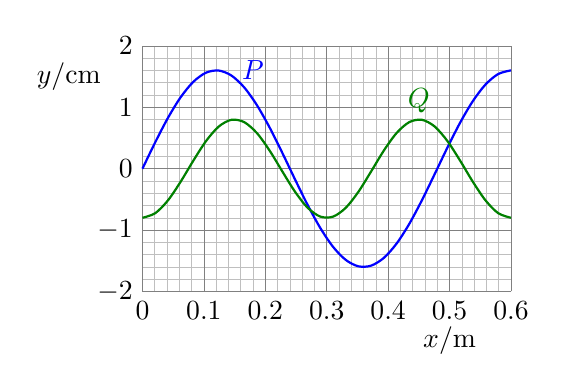
\begin{tikzpicture}[scale=0.78]
	\draw[help lines, gray!50, very thin, step=0.2] (0,-2) grid (6,2);
	\draw[help lines, step=1] (0,-2) grid (6,2);
	\foreach \y in {-2,-1,0,1,2} \node[left] at (0,\y) {$\y$};
	\foreach \x in {0,0.1,0.2,0.3,0.4,0.5,0.6} \node[below] at (10*\x,-2) {$\x$};
	\node at (-1.2,1.5) {$y$/cm};
	\node at (5,-2.8) {$x$/m};
	\draw [thick, blue, domain=0:6, samples=30, smooth] plot (\x,{1.6*sin(75*\x)});
	\draw [thick, Green, domain=0:6, samples=30, smooth] plot (\x,{-0.8*cos(120*\x)});
	\node[blue] at (1.8, 1.6) {$P$};
	\node[Green] at (4.5, 1.1) {$Q$};
	\end{tikzpicture}
	\vspace*{-18pt}
\end{marginfigure}

\question{The graph shows the variation of displacement $y$ with the distance $x$ of wave $P$ and wave $Q$ at some instant. (a) For each of the two waves, state the amplitude and the wavelength. (b) Given that both waves have a time period of 0.30 s, find the frequency of the waves, and hence find the speed for each wave.}


\subsection*{transverse \& longitudinal waves}

\question{
	An ultrasound waves of frequency 2.0 MHz travels with a speed of $1600 \mps$ through water. What is the shortest distance from a point of maximum pressure to a point of	minimum pressure?
}

\begin{marginfigure}
	\vspace*{-12pt}
	\centering
	\begin{tikzpicture}[xscale=0.6,yscale=0.75]
	\draw [->] (0,-2) -- (0,2.4) node[midway,left]{$O$} node[left]{$y$};
	\draw [->] (0,0) -- (2.5*pi,0) node[below]{$x$};
	\draw[very thick,->] (1.6*pi,2) -- (2.4*pi,2);
	\node[above,twoline] at (2*pi, 2.2) {direction of\\wave motion};
	\draw [thick, blue, domain=0:2.4*pi, samples=30, smooth] plot (\x,{1.6*sin(\x*1.2 r)});
	\draw[fill, red] (5*pi/12,1.6) circle (0.08) node[above, black]{$P$};
	\draw[fill, red] (10*pi/12,0) circle (0.08) node[above right, black]{$Q$};
	\draw[fill, red] (15*pi/12,-1.6) circle (0.08) node[below, black]{$R$};
	\draw[fill, red] (20*pi/12,0) circle (0.08) node[above left, black]{$S$};
	\end{tikzpicture}
	\vspace*{-16pt}
\end{marginfigure}

\question{
	The graph shows the variation with distance $x$ of the displacement $y$ of a wave on a stretched rope at
	time $t = 0$. The wave has a frequency of 1.0 Hz. (a) State and explain whether this wave is transverse or longitudinal. (b) For the points $P$, $Q$, $R$, and $S$ labelled on the graph, which one of them is moving upwards with greatest speed at $t=0$? (c) Sketch the wave pattern at $t = 0.50 \text{ s}$. (c) For the points $P$, $Q$, $R$, and $S$, what are their positions at $t = 0.50 \text{ s}$?
}


\question{
	Given a slinky toy, suggest how you can demonstrate (a) a transverse wave, (b) a longitudinal wave to your classmates.
}

\subsection*{sound waves}

\question{
	If some alien civilisation blows up the moon one day, can we hear it?
}

\question{An oscilloscope is used to measure a sound wave. When the time base is set at 5.0 ms div$^{-1}$, 3 complete waveforms are observed over 5 divisions. Calculate, (a) the period of the wave, (b) the frequency of the wave.}

\question{Describe the changes to the wave pattern displayed on an oscilloscope if the sound being measured has (a) a higher pitch, (b) a greater volume.}


\subsection*{electromagnetic waves}

\question{
	Green light has a wavelength of 500 nm in vacuum. What is its frequency?
}

\question{
	An electromagnetic wave has a period of 1.0 ps. (a) What is the wavelength of this wave? (b) What is the number of wavelengths in a distance of 1.0 m?
}

\question{
	(a) What is the frequency of the longest-wavelength ultraviolet wave? (b) What is the frequency of the shortest-wavelength infra-red radiation?
}

\question{
	State a typical value for the wavelength for the following radiation in vacuum: (a) infra-red, (b) X-ray, (c) microwave, (d) ultraviolet.
}

\question{
	A student argues that the speed of an electromagnetic wave is proportional to its frequency because we have $c=\lambda f$. State and explain whether the student's argument is correct.
}

\question{
	(a) Suggest as many properties of electromagnetic waves as you can. (b) Among these properties you have listed, which property of electromagnetic wave is distinct from other transverse waves?
}

%\question{
%	Suppose a sound wave and an electromagnetic wave have the same wavelength, compare their frequencies.
%}

\subsection*{intensity of waves}

\question{
	A sound wave in air has an amplitude $A_0$ and intensity $I_0$. If the amplitude increases to $3A_0$, what is the new intensity?
}

\question{
	The intensity of radiation arriving normally on a solar panel was $500 \text{ W m}^{-2}$. (a) If the panel has an effective area of $4.0 \text{ m}^2$, how much energy would arrive in one hour? (b) If the radiation has double the amplitude, how much energy would arrive in one hour?
}

\question{
	The intensity $I$ of a sound wave can be given by the formula: $I = k v \rho f^2 A^2$, where $v$ is the speed of sound, $\rho$ is the density of the medium, $f$ is the frequency and $A$ is the amplitude. Show that $k$ is a unit-free constant.
}



\question{
	A point source gives out spherical waves. How does the wave amplitude $A$ vary with the distance $r$ from the source?
}

\subsection*{polarisation}

\question{
	A horizontally polarised beam of light of intensity $I_0$ passes through a polarising filter whose plane of polarisation is at $30^\circ$ to the horizontal. What is the transmitted intensity?
}

\question{
	When polarized light is sent through some chemical solution, the plane of polarization is rotated. If the intensity is $I$ without the solution being placed in the beam but $0.80I$ after the sugar is placed in the beam, what is the angle of rotation?
}

\question{
	A beam of unpolarised light is sent through two polarising filters $A$ and $B$. Filter $A$ has its axis of
	polarisation in the vertical direction, and filter $B$ has its axis of polarisation in the horizontal direction. (a) What is the emergent intensity? (b) A third polarising filter $C$ is inserted between the filters $A$ and $B$, such that filter $C$ has its plane of polarisation at an angle of $45^\circ$ to the vertical. What is the new emergent intensity?
}

\question{
	Suggest how you may use a stretched elastic rope to demonstrate the phenomenon of polarisation.
}

\subsection*{diffraction}

\question{
	A hill stands between a house and a radio transmitter, but radio signals sent from the transmitter are still received at the house. How can this happen?
}

\question{
	Diffraction can be demonstrated by observing how water waves in a ripple tank go through a gap. Suggest whether the following action would lead to greater or less obvious diffraction: (a) increasing the frequency of the water waves, (b) increasing the amplitude of the waves, (c) increasing the width of the gap, (d) increasing the speed of the waves by increasing the depth of water.
}

\question{
	Microwave ovens use microwaves of frequency of around 2.4 GHz to heat food. The front door of many microwave ovens is made of glass with a metal grid, where gap in the grid are a few mm across. By reference to the wavelength of the microwave, explain how the front door keeps microwaves in but could let light out.
}

% \subsection*{Doppler effect}

% For the questions below, take the speed of sound to be $340 \mps$. 

% \question{A car travels with a constant speed along a straight road. The car's horn is known to sound at a frequency of 500 Hz, but an observer standing on the roadside hears a frequency of 450 Hz. What is the magnitude and the direction of the car's velocity relative to the observer?}


% \question{
% 	An ambulance travelling at a steady speed of $25 \mps$ passes close to a stationary observer. The warning signal on the ambulance has a frequency of 1500 Hz. What is the overall change in the frequency heard by the observer as the ambulance goes by?
% }

% \question{
% 	If the motion of the source is at right angles to an observer, state and explain whether there will be a Doppler effect?
% }


% \question{
% 	A girl sits on a horizontal platform that is rotating about a vertical axis. The girl moves in a circular path with a constant speed of $8.0 \mps$. The girls starts blowing a whistle which emits a sound of frequency 1200 Hz. To an observer standing at a distance, (a) find the maximum and the minimum frequency heard. (b) Describe the variation in the frequency of the sound heard by the observer.
% }

% \question{
% 	A spectral line of a particular wavelength is emitted from a distant star. The wavelength observed is found to vary periodically from a maximum value to a minimum value and back to the maximum value. What can you say about the motion of the star?
% }



% \question{
% 	[This question is beyond CAIE syllabus] (a) A source emits sound wave of frequency $f$. If the observer, rather than the source, is in motion, suggest whether there is any change in the apparent frequency $f^\prime$ heard by the observer. (b) If the observer is moving towards the source at a velocity of $v_o$, show that the observed frequency $f'$ is: $f' = f \frac{v+v_o}{v}$. (c) If the observer is moving away from the source, derive a similar expression for the observed frequency. 
% }
